\documentclass[a4paper,12pt]{jarticle}
\input ./chap01_preamble.tex
\graphicspath{%
  {../text01-img/}%
}
% !TEX root = ./chap01_01.tex
\begin{document}
\section{今回の\ruby{授業}{じゅぎょう}}
\subsection{目標}
\ \ \ \ ラズベリーパイになれよう

\ \ \ \ 自分のホームページを作れるようになろう

\subsection{\ruby{授業内容}{じゅぎょうないよう}}
%\liststyleLii
\begin{enumerate}
  \item ラズベリーパイとは
  \item ラズベリーパイになれよう(1)
  \item ラズベリーパイになれよう(2)
  \item 自分の\ruby{紹介}{しょうかい}ページを作ろう
\end{enumerate}
\subsection{注意点}
%\liststyleLiii
\begin{itemize}
  \item
      \ruby{授業}{じゅぎょう}の合間のきゅうけいでは、遠くのものをながめたりして目を休めましょう
  \item 水分ほきゅうはこまめにしましょう
  \item
        先生が説明中は先生の話を聞きましょう
  \item
        わからないことがあったらTAの先生方にすぐ聞きましょう
\end{itemize}
\subsection{教科書について}
%\liststyleLiv
\begin{itemize}
  \item
        教科書には例題、それに\ruby{似}{に}た問題があります。まずは、例題をよく読みながら試してみましょう。そのあと問題を\ruby{解}{と}きましょう。問題の答えは一番最後のページにあります。
\end{itemize}
\clearpage\subsection{\ruby{配布物}{はいふぶつ}の\ruby{確認}{かくにん}}

\bigskip

%\liststyleLv
\begin{enumerate}
  \item ラズベリーパイ
  \item SDカード(16GB)
  \item でんげんケーブル
  \item HDMIケーブル
  \item GPIOエクステンダー
  \item ヘッドセット
  \item マウス
  \item センサーボード
  \item ウェブカメラ
  \item ディスプレイ(持って帰れません)
\end{enumerate}
\clearpage

\begin{tabular}{cc}
  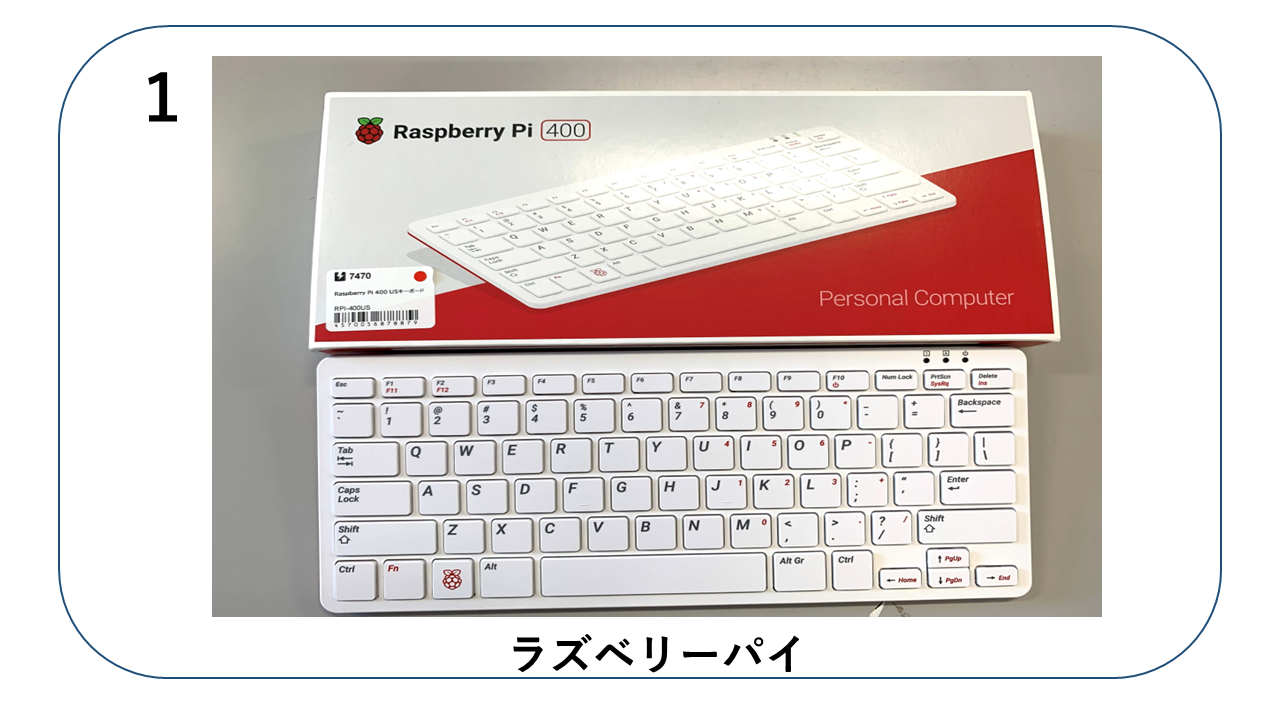
\includegraphics[width=6.488cm,height=4.697cm]{textbook-img009-2023.png}
   &
  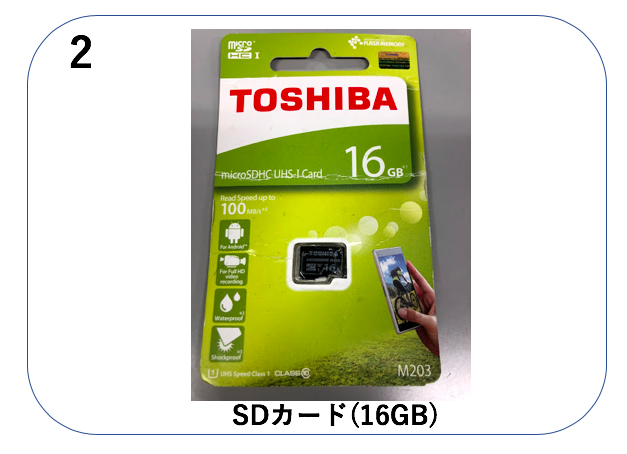
\includegraphics[width=6.488cm,height=4.697cm]{textbook-img010.png} \\

  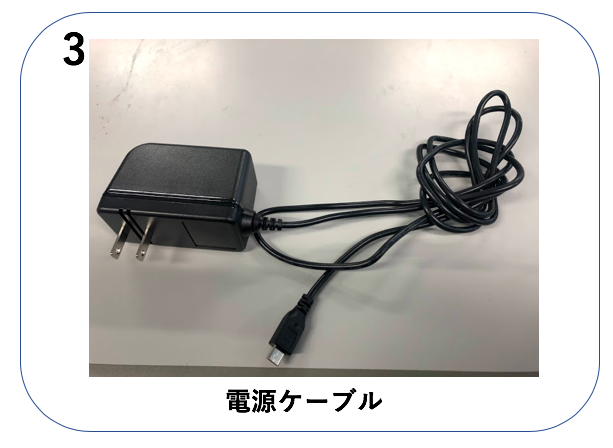
\includegraphics[width=6.488cm,height=4.697cm]{textbook-img007.png}
   &
  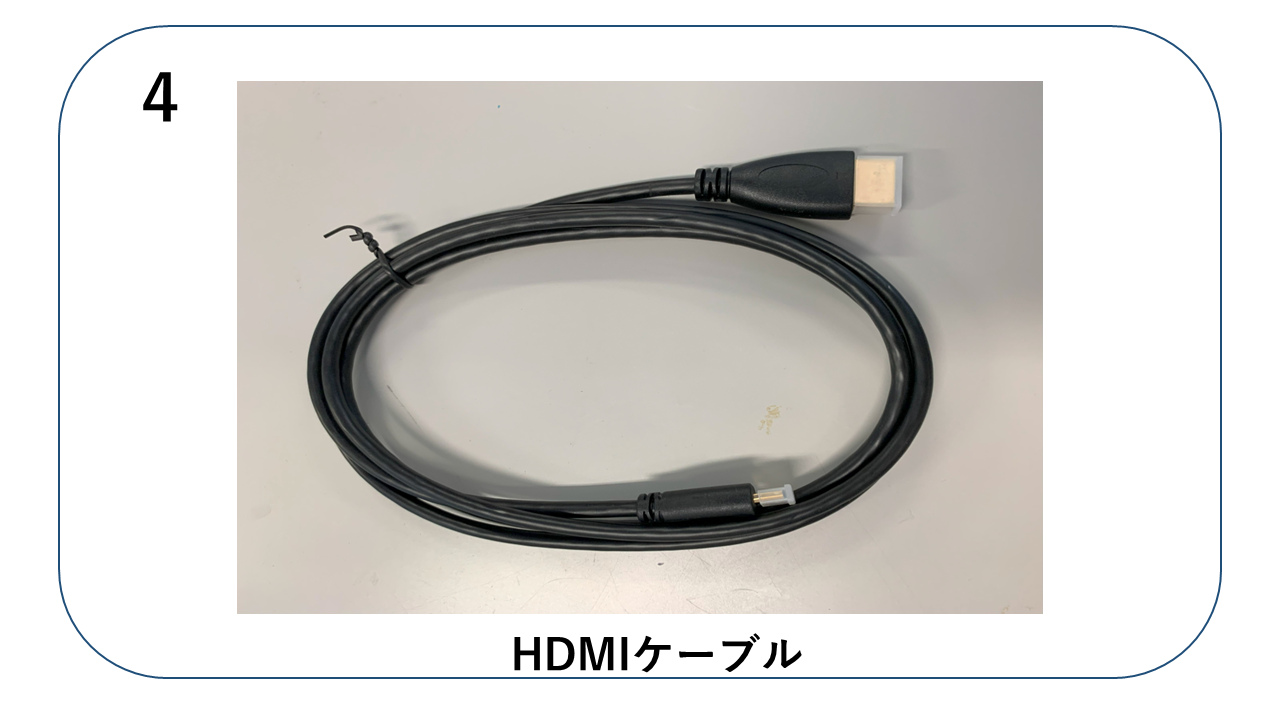
\includegraphics[width=6.488cm,height=4.697cm]{textbook-img008-2023.png} \\

  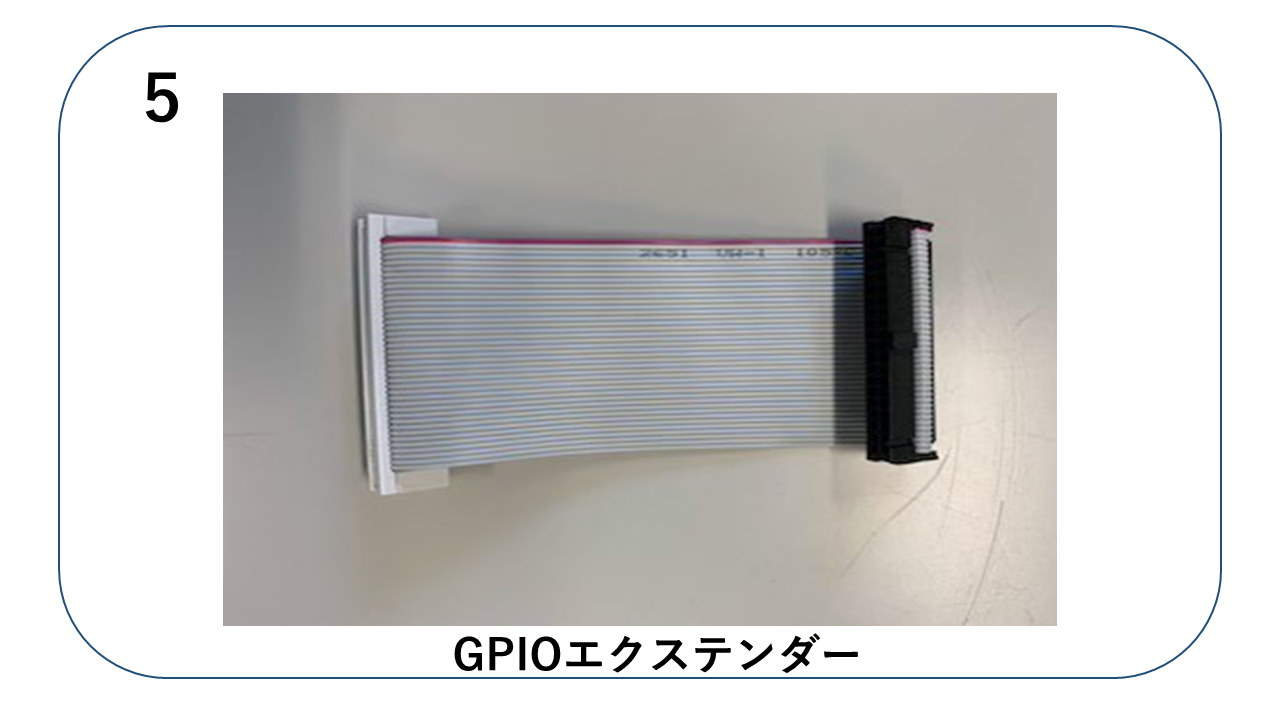
\includegraphics[width=6.488cm,height=4.697cm]{textbook-img005-2023.png}
   &
  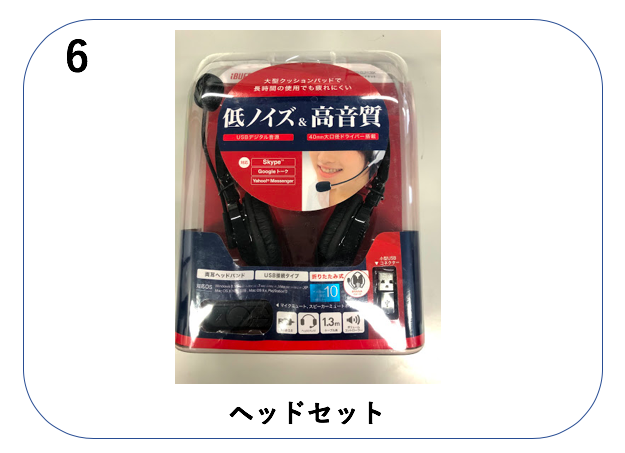
\includegraphics[width=6.488cm,height=4.697cm]{textbook-img006.png} \\

  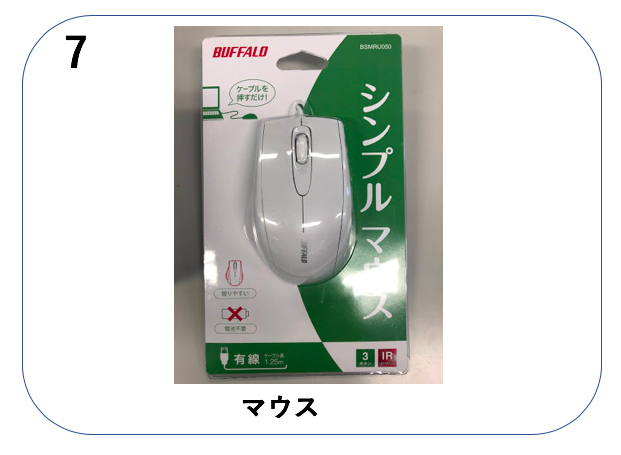
\includegraphics[width=6.488cm,height=4.697cm]{textbook-img003.png}
   &
  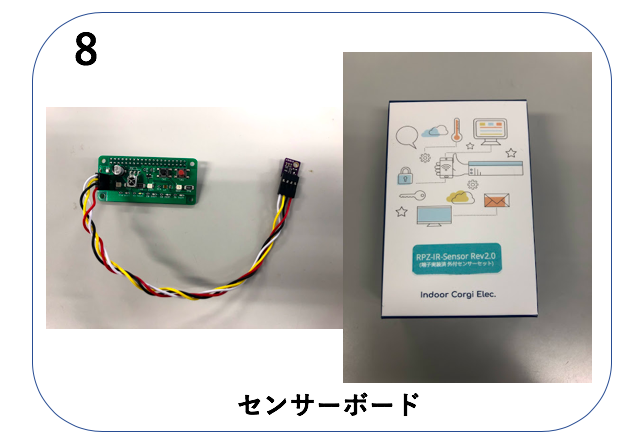
\includegraphics[width=6.488cm,height=4.697cm]{textbook-img004.png} \\

  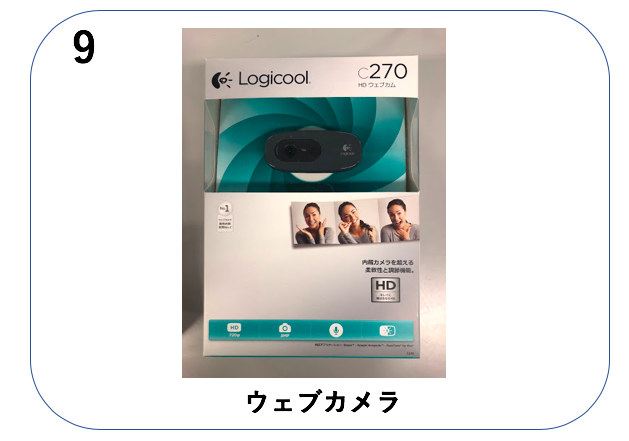
\includegraphics[width=6.488cm,height=4.697cm]{textbook-img002.png}
   &
  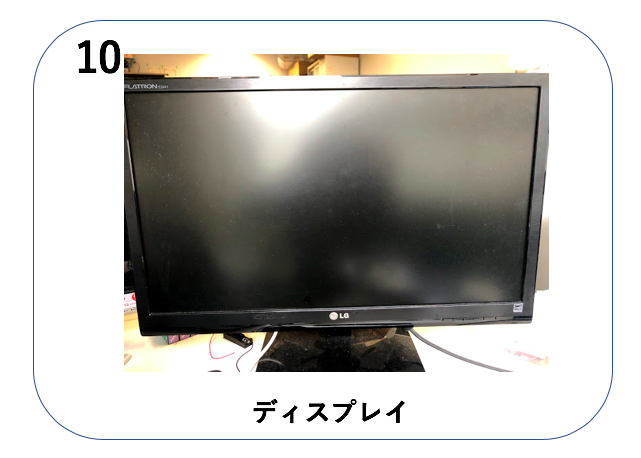
\includegraphics[width=6.488cm,height=4.697cm]{textbook-img001.png} \\
\end{tabular}

%\liststyleLv\ruby{}
\subsection{ラズベリーパイについて}
イギリスのラズベリーパイ\ruby{財団}{ざいだん}というグループが開発したコンピュータです。いろいろな\ruby{種類}{しゅるい}がありますが、子供IT\ruby{未来塾}{みらいじゅく}ではキーボード一体型タイプのラズベリーパイを使用しています。ラズベリーパイは短くラズパイとも\ruby{呼}{よ}ばれています。

\subsection{\ruby{特徴}{とくちょう}}
%\liststyleLvi
\begin{itemize}
  \item キーボード一体型で、キーボードが必要ない
  \item \ruby{普通}{ふつう}のパソコンのように使える
  \item (動画\ruby{再生}{さいせい}やゲームもできます)
  \item
        プログラミングのべんきょうに向いている
  \item
        モータやライトをせいぎょできる(目に見えるのでプログラミングを楽しめる)
\end{itemize}
\subsection{ラズベリーパイでできること}
プログラミングを手軽に学ぶことができます。プログラミングをするときにはパソコンが必要

でお金もかかりやりたくてもできないひともいたかもしれません。しかし、ラズベリーパイの

ような小さくて手に入れやすいコンピュータがあれば手軽にプログラミングの学習に取り組む

ことができます。また、ラズベリーパイを使うことでモータやライトなどを動かしたり光らせ

たりすることができます。これらのせいぎょをプログラムで行うことができるので楽しみなが

ら学習を進められます。

\subsection{ラズベリーパイを使うときの注意}
%\liststyleLvii
\begin{itemize}
  \item
        水などぬれているものをラズベリーパイ本体につけないようにしましょう
\end{itemize}
%\liststyleLviii
\begin{itemize}
  \item
        ラズベリーパイをはじめコンピュータなどは熱に弱いのですごく暑い部屋では使わないようにしましょう
\end{itemize}
%\liststyleLix
\begin{itemize}
  \item
        ラズベリーパイなどは静電気によわいので注意しましょう
\end{itemize}
%\liststyleLx
\begin{itemize}
  \item
        ラズベリーパイをらんぼうに\ruby{扱}{あつか}うのはやめましょう
\end{itemize}


\clearpage
\subsection{パスワードについて学ぼう}
\begin{enumerate}
  \item
  パスワードの\ruby{重要性}{じゅうようせい}について知ろう
      \begin{itemize}
      \item
          IDとパスワードは、タブレットやパソコンなどの\ruby{情報機器}{じょうほうきき}や、インターネット上のサービスを利用する\ruby{際}{さい}に、\ruby{許可}{きょか}された者であるかを\ruby{識別}{しきべつ}し、本人を\ruby{確認}{かくにん}するための重要な\ruby{情報}{じょうほう}です。 いわゆるインターネットやパソコンなどの電子機器に入るための\ruby{鍵}{かぎ}の名前(ユーザーID)とその\ruby{鍵}{かぎ}(パスワード)のようなものです。
          \begin{figure}[h]
            \centering
            \begin{minipage}{5.228cm}
              {\upshape
                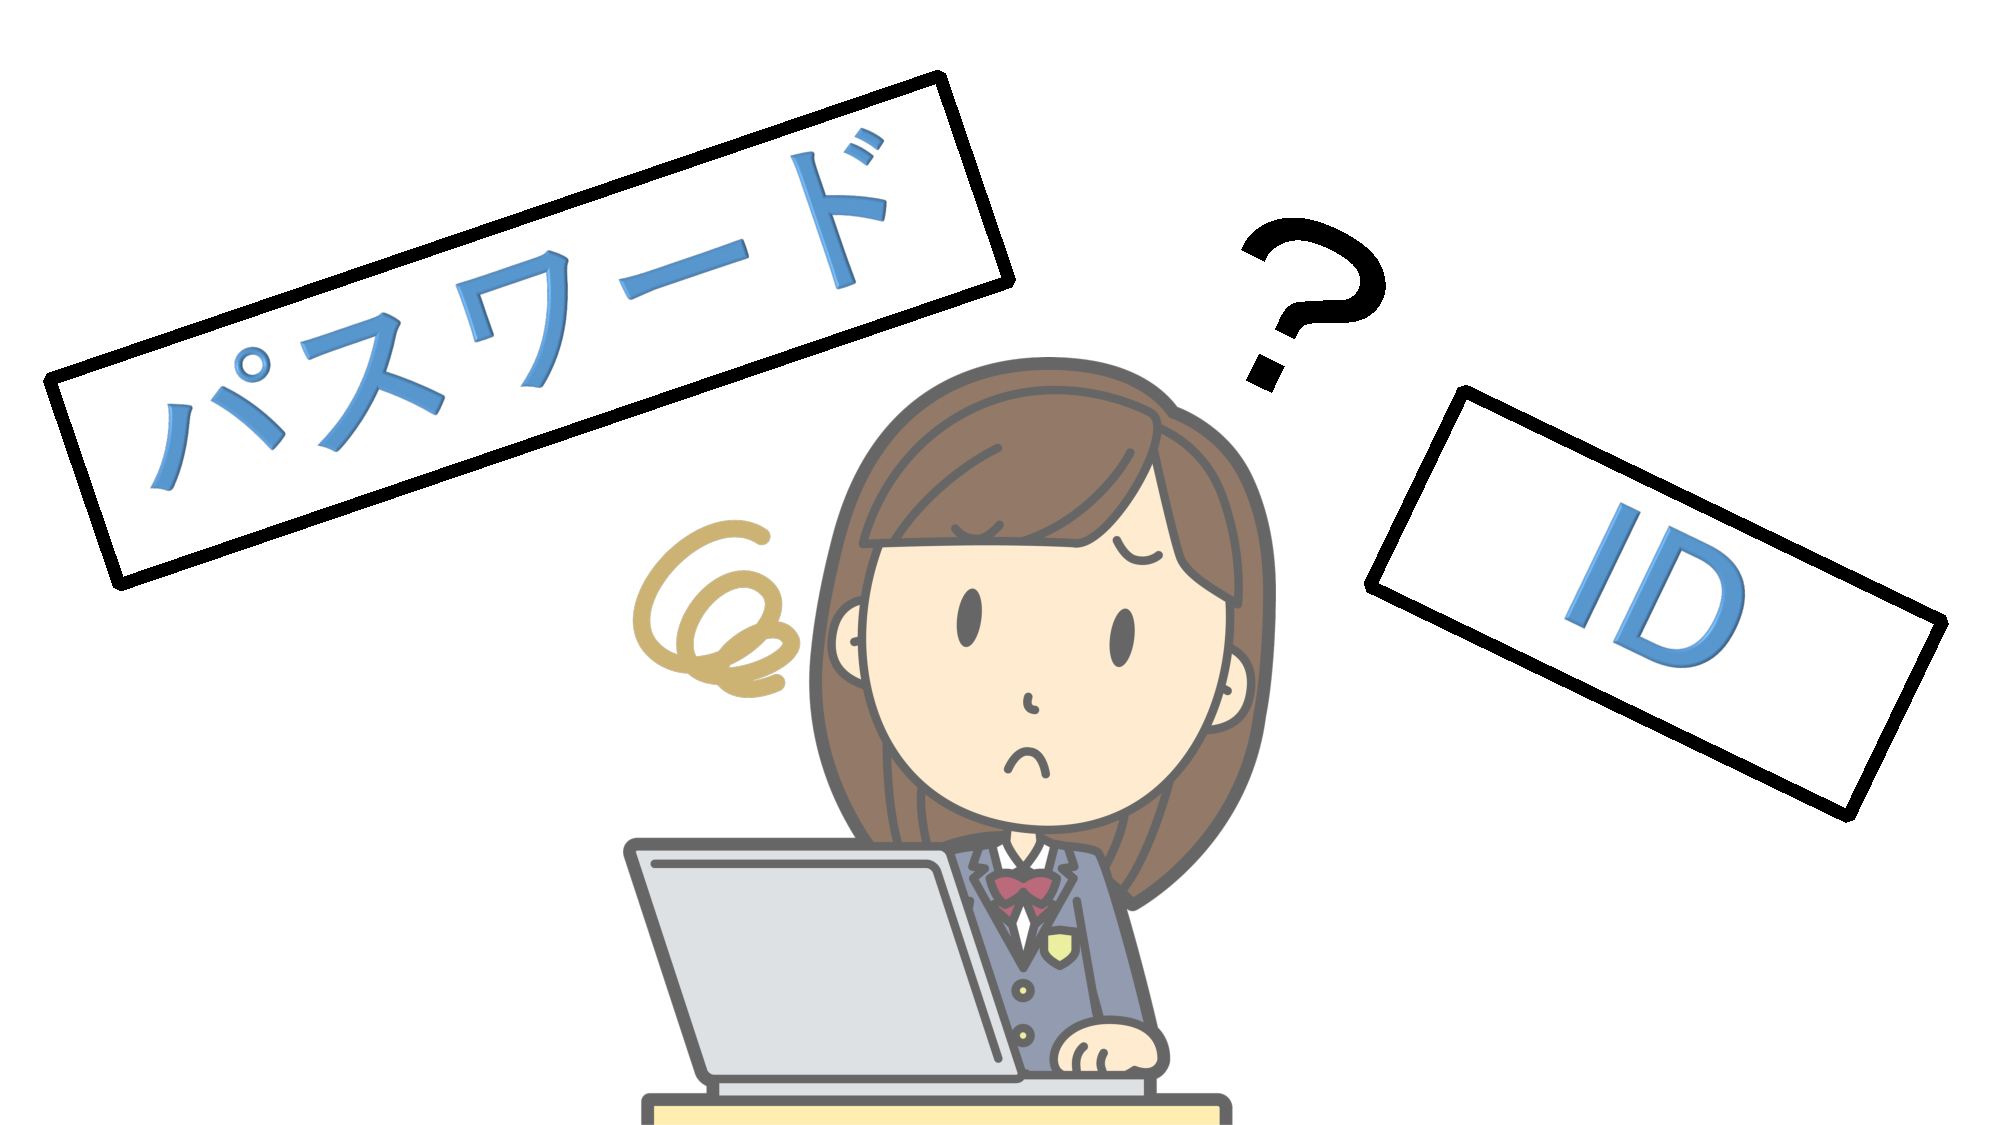
\includegraphics[width=7.000cm]{pswd_image_imp6.pdf}
                }
            \end{minipage}
          \end{figure}
          \item
              IDやパスワードなど\ruby{認証}{にんしょう}で使っている\ruby{情報}{じょうほう}(\ruby{身分証明書}{みぶんしょうめいしょ})を\ruby{不適切}{ふてきせつ}な管理や、\ruby{攻撃}{こうげき}などで\ruby{盗}{ぬす}まれてしまうと、なりすましなどの\ruby{不正行為}{ふせいこうい}が行われてしまう\ruby{危険性}{きけんせい}もあります。
          \begin{figure}[h]
            \centering
              \begin{minipage}{5.228cm}
                {\upshape
                  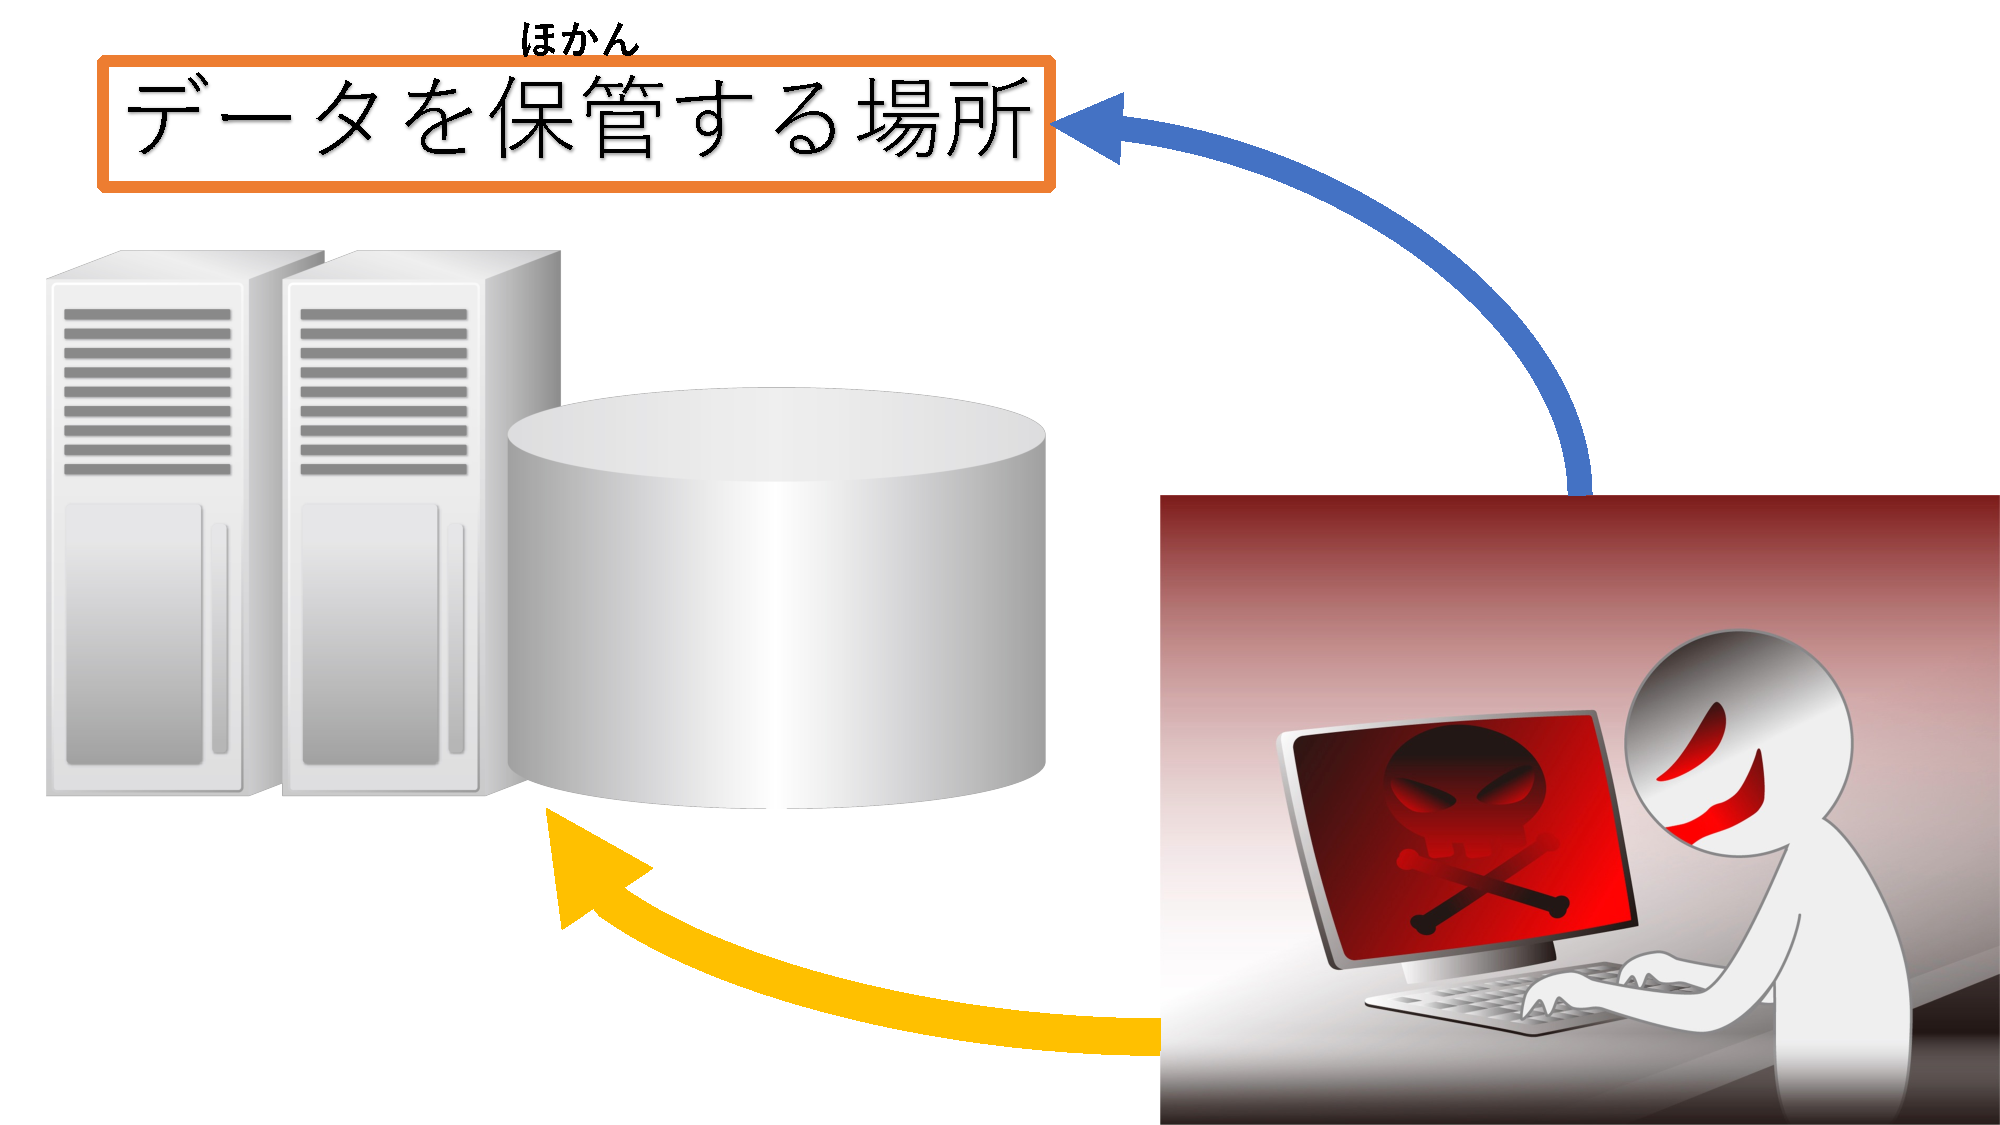
\includegraphics[width=7.000cm]{pswd_image_imp5.pdf}
                  }
              \end{minipage}
            \end{figure}
          \item
              このような手口による\ruby{被害}{ひがい}にあわないように\ruby{認証}{にんしょう}の仕組みと\ruby{重要性}{じゅうようせい}を\ruby{理解}{りかい}しIDやパスワードを\ruby{厳重}{げんじゅう}に管理しましょう。
          \begin{figure}[h]
          \centering
            \begin{minipage}{5.228cm}
              {\upshape
                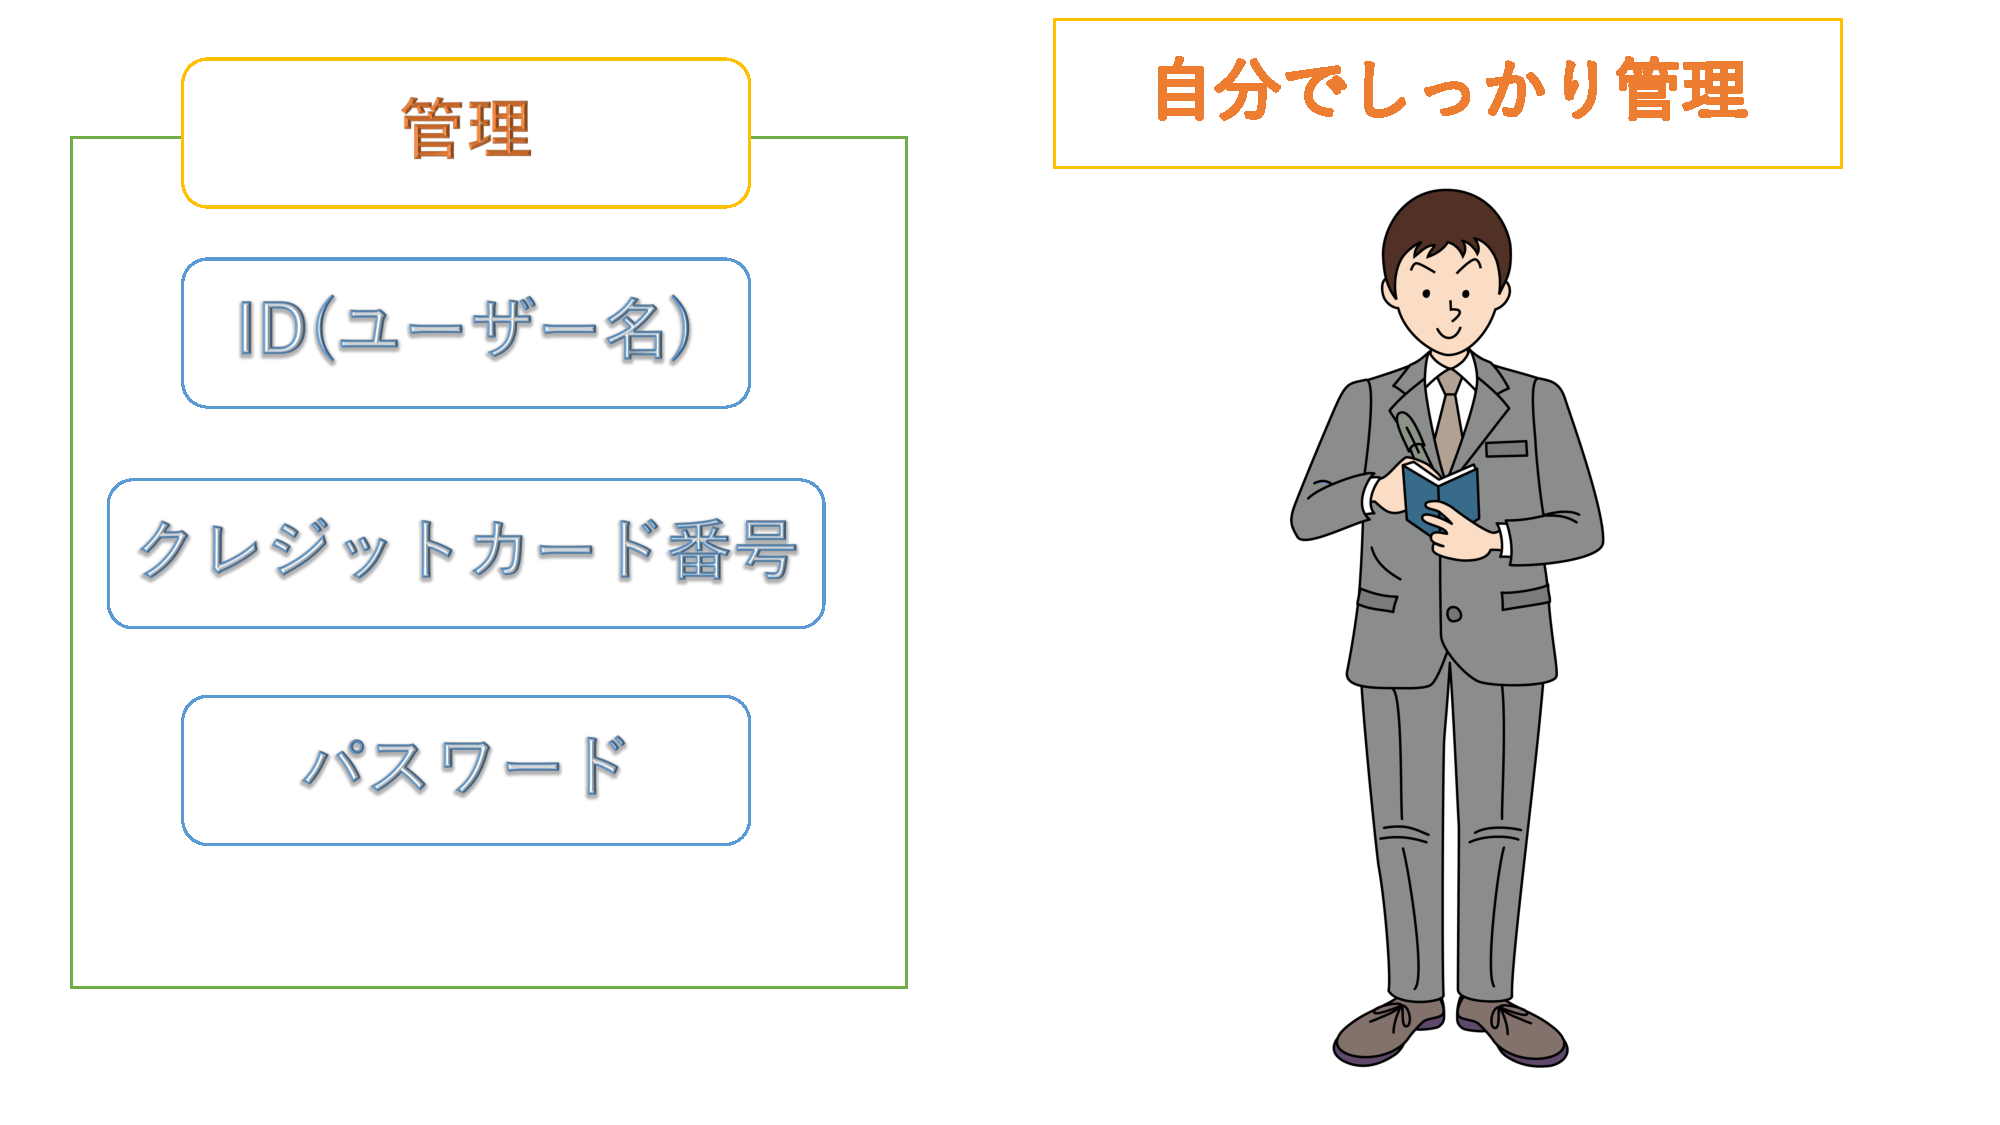
\includegraphics[width=7.000cm]{pswd_image_imp3.pdf}
                }
            \end{minipage}
          \end{figure}


\end{itemize}


\clearpage
  \item
          安全なパスワードの\ruby{設定}{せってい}やパスワードの\ruby{適切}{てきせつ}な管理について知ろう。
          
      \begin{itemize}
        
          \item
                安全なパスワードとは他人に\ruby{推測}{すいそく}されにくく、計算で\ruby{割}{わ}り出しにくいものです。
          \begin{itemize}
            \item 
              名前などの\ruby{個人情報}{こじんじょうほう}からは\ruby{推測}{すいそく}できないこと
              \item   
              英単語などをそのまま使用していないこと
              \item   
              アルファベットと数字が\ruby{混在}{こんざい}していること
              \item 
              \ruby{適切}{てきせつ}な長さの文字列であること
              \item 
              \ruby{類推}{るいすい}しやすい\ruby{並}{なら}び方やその\ruby{安易}{あんい}な組合せにしないこと
            \end{itemize}
                \begin{figure}[h]
                  \centering
                  \begin{minipage}{5.228cm}
                    {\upshape
                      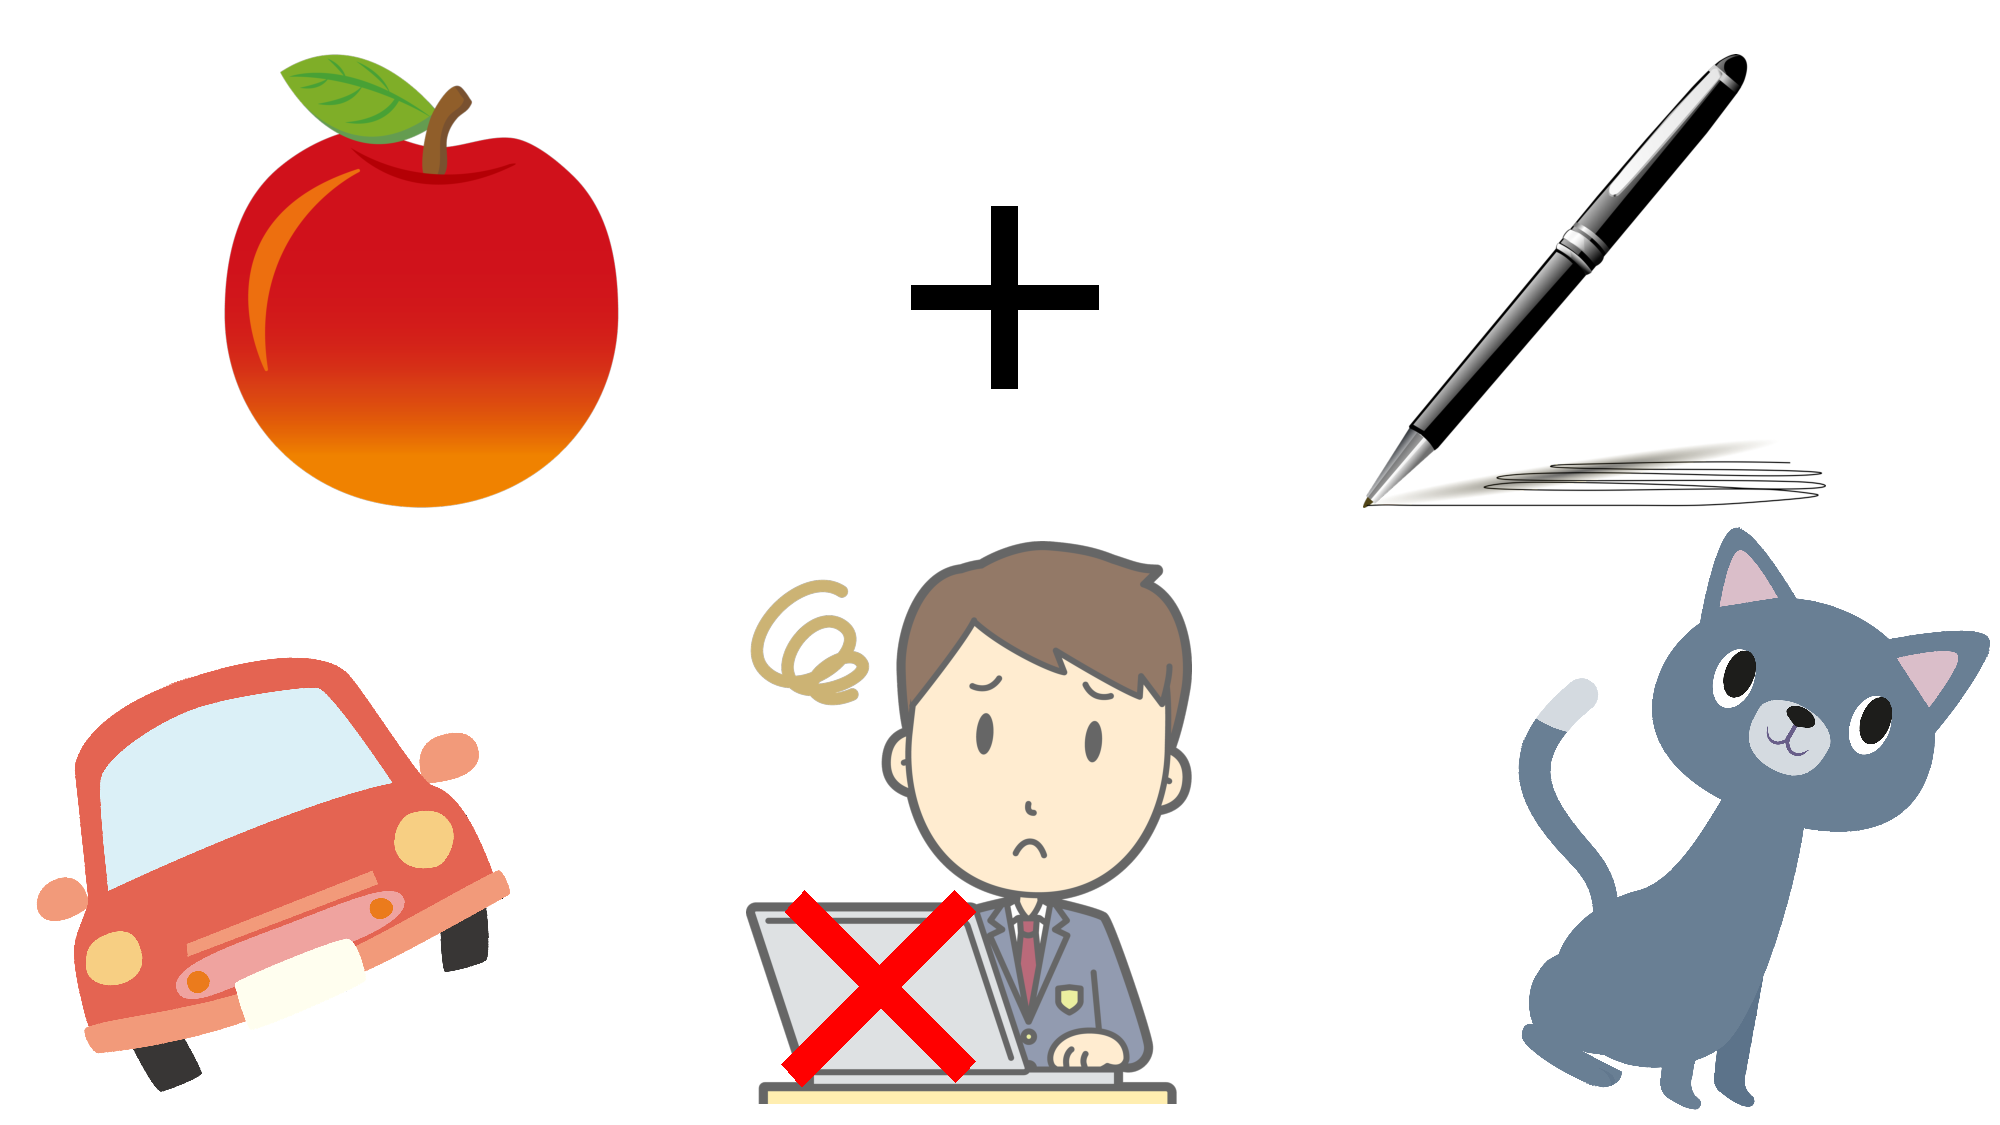
\includegraphics[width=7.000cm]{pswd_image_imp11.pdf}
                      }
                  \end{minipage}
                  \end{figure}  
             \item   パスワードはできる限り、\ruby{複数}{ふくすう}のサービスで使い回さないようにしましょう。またパスワードを定期的に\ruby{変更}{へんこう}することを求められても、\ruby{実際}{じっさい}にパスワードを\ruby{破}{やぶ}られアカウントが乗っ取られたり、サービス側から流出した事実がなければパスワードを\ruby{変更}{へんこう}する必要はありません。
                     
          \begin{figure}[h]
            \centering
            \begin{minipage}{5.228cm}
              {\upshape
                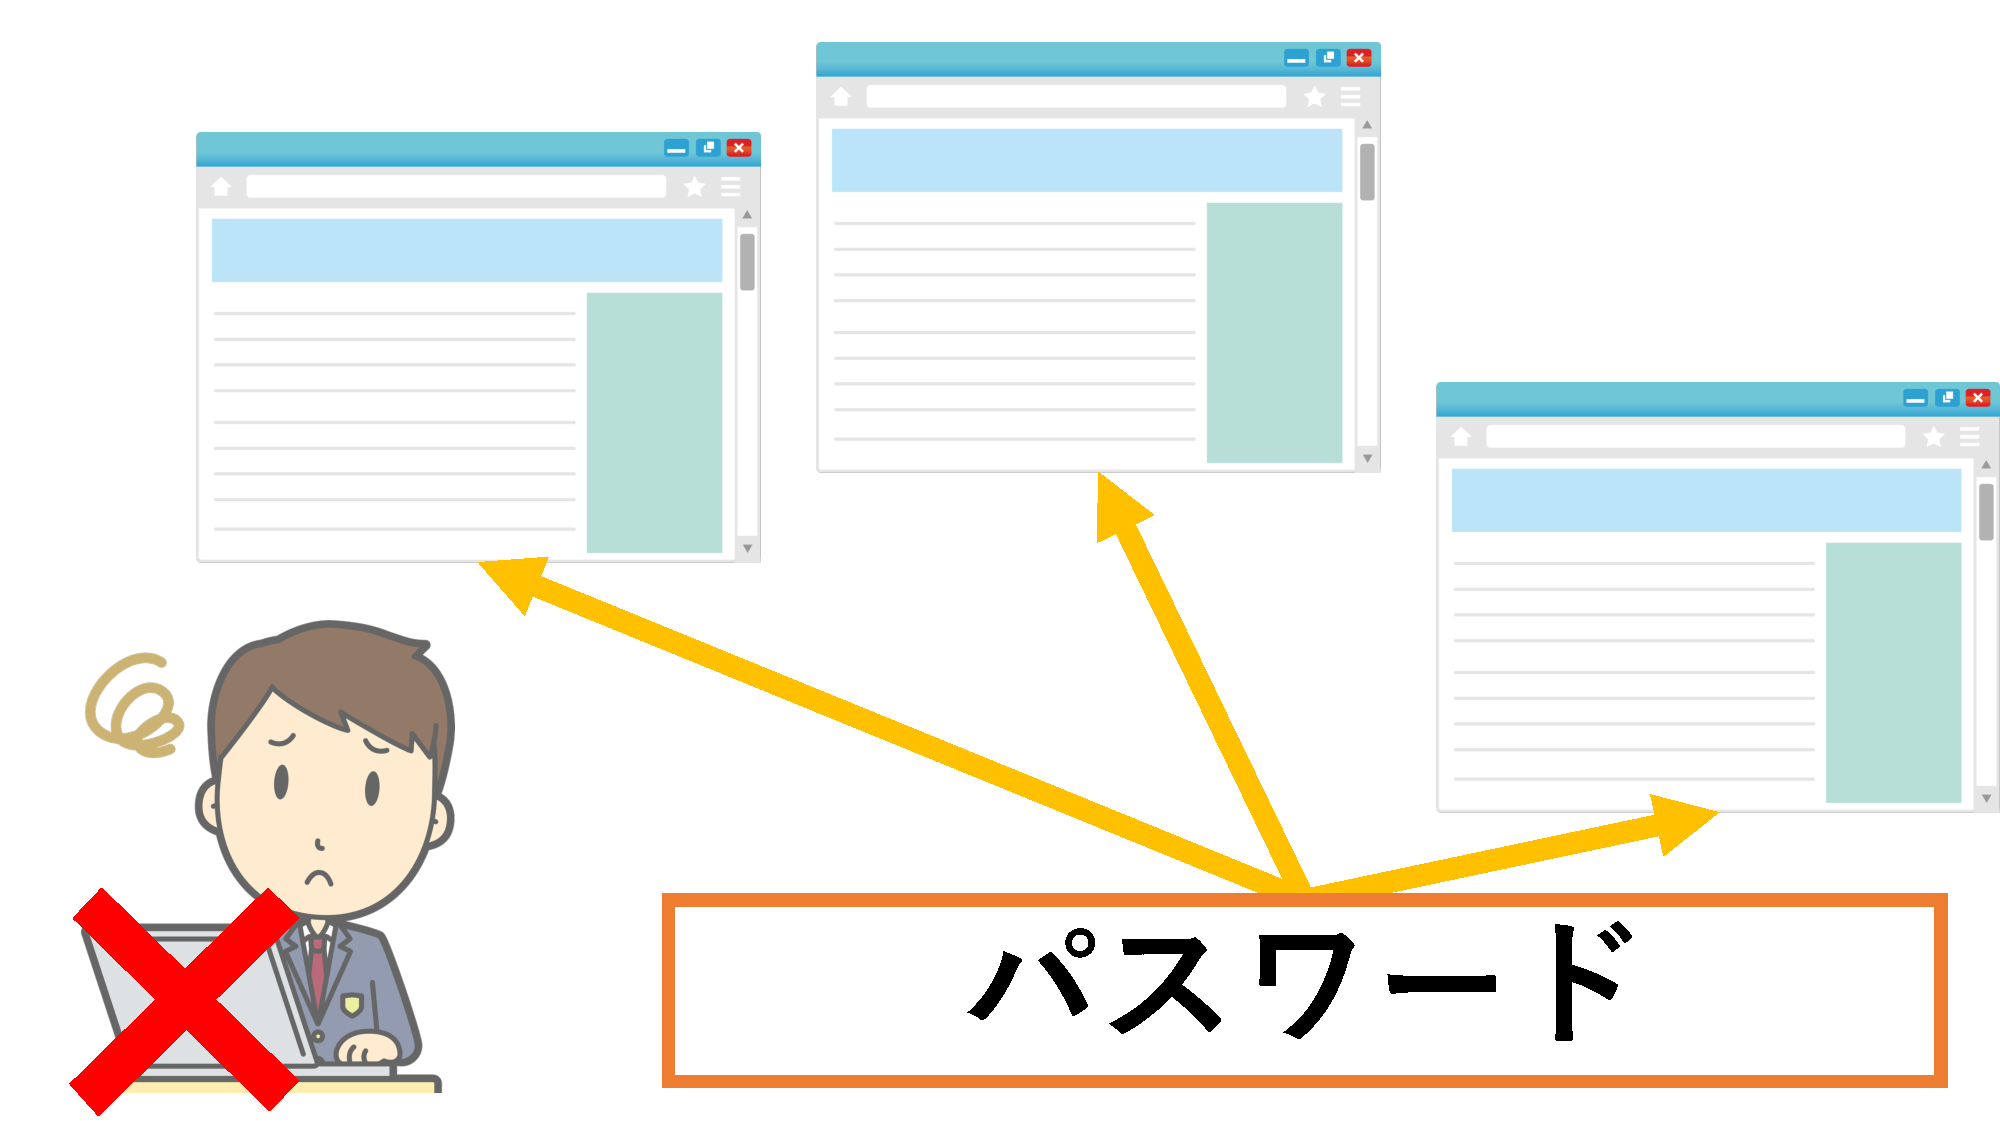
\includegraphics[width=7.000cm]{pswd_image_imp10.pdf}
                }
            \end{minipage}
            \end{figure}
              \item
                安全なパスワードを\ruby{設定}{せってい}してもパスワードが他人に\ruby{漏}{も}れてしまえば意味がありません。以下に関して特に\ruby{留意}{りゅうい}が必要です。
            \begin{itemize}
              \item
                    パスワードは友人などに教えずに\ruby{秘密}{ひみつ}にすること
              \item      
                    パスワードをメールやSNSなどでやりとりしないこと
              \item       
                    パスワードのメモなどを他人の目に付く場所に\ruby{貼}{は}ったり置いたりしないこと
              \item 
                    パスワードをメモした場合は\ruby{鍵}{かぎ}のかかる\ruby{机}{つくえ}や金庫など安全に\ruby{保管}{ほかん}すること                     
            \end{itemize}
              \item
              出典: \ruby{総務省}{そうむしょう}『国民のための\ruby{情報}{じょうほう}セキュリティサイト』\url{https://www.soumu.go.jp/main_sosiki/joho_tsusin/security/basic/privacy/01-1.html}を加工して作成
      \end{itemize}
          \clearpage
          \item パスワードの\ruby{制限}{せいげん}について知ろう
          \begin{itemize}
            \item
                  Linuxのユーザー名とパスワードの\ruby{入力基準}{にゅうりょくきじゅん}において以下の\ruby{条件}{じょうけん}があります。
                  \begin{itemize}
                  \item
                          ユーザー名は小文字、数字、-、のみ使用\ruby{可能}{かのう}。
                    \item
                        パスワードは8文字以上16文字以下。
                    \item
                        パスワードには以下の四つのカテゴリタイプの文字の内、三つのカテゴリタイプの文字を入れる必要がある。
                  \end{itemize}
          \end{itemize}
          \begin{table}[htbp]
            \centering
            \caption{文字タイプ表}
            \begin{tabular}{|c|c|}
            \hline
                タイプ & \ruby{実際}{じっさい}に使用\ruby{可能}{かのう}な文字 \\
                \hline
                大文字& ABCDEFGHIJKLMNOPQRSTUVWXYZ\\
                \hline
                小文字& abcdefghijklmnopqrstuvwxyz\\
                \hline
                数字 &0123456789\\
                \hline
                英数字以外の文字&~!@\#\$\%\textasciicircum\&*()\_+`\{\}\textbar[]\textbackslash:";'\textless\textgreater?,./\\
                \hline
            \end{tabular}
            \end{table}
          \begin{itemize}
              \item
                  \ruby{注意事項}{ちゅういじこう}
                  \begin{itemize}
                  \item
                      パスワードの先頭の大文字とパスワードの\ruby{末尾}{まつび}の数字は、使用される文字クラスの数にはカウントされません。
                  \item
                  パスワードには辞書の単語やユーザーのログイン名を\ruby{含}{ふく}めることはできません。
                  \item
                  文字を数字または英数字以外の文字に置き\ruby{換}{か}えると、辞書の単語が受け入れられるようになります。(例)app1e, ta2ya
                  \item
                  自分が覚えやすいものになるべくしてください。※\ruby{公}{おおやけ}になっている\ruby{羅列}{られつ}やその他ですでに使用しているものは\ruby{避}{さ}けてください。
                  \end{itemize}
          \end{itemize}
          \begin{itemize}
              \item
                  \refstepcounter{Question}\theQuestion 得た\ruby{知識}{ちしき}を\ruby{踏}{ふ}まえてパスワードとユーザ名を決めて下の\ruby{記入欄}{きにゅうらん}に記入してみましょう。
                  \addBlank{ユーザ名(ID)}
                  \addBlank{パスワード}
          \end{itemize}
          
          \clearpage


          \begin{itemize}   
                        \item
                            \refstepcounter{Question}\theQuestion\label{Q:hasAnswer01-2} 次の文章の\ruby{間違}{まちが}っている部分を訂正してください。また{間違}{まちが}っている部分が無い場合は×を記入してください。
                          
                          \begin{enumerate}[label=\textbf{(\arabic*)}]
                          \item  名前などの\ruby{個人情報}{こじんじょうほう}からは\ruby{推測}{すいそく}でしやすい方が良い
                          \item  英単語などをそのまま使用して良い
                          \item \ruby{適切}{てきせつ}な長さの文字列である方が良い
                          \item \ruby{類推}{るいすい}しやすい\ruby{並}{なら}び方やその\ruby{安易}{あんい}な組合せが良い
                          \end{enumerate}
                        \begin{table}[htbp]
                          \centering
                          
                          \begin{tabular}{|c|c|c|}
                          \hline
                              番号&\ruby{訂正}{ていせい}する\ruby{箇所}{かしょ}&\ruby{訂正後}{ていせいご}  \\
                              \hline
                              例(1)& \ruby{推測}{すいそく}しやすい&\ruby{推測}{すいそく}しにくい\\
                              \hline
                              (2)& & \\
                              \hline
                              (3)& & \\
                              \hline
                              (4)& & \\
                              \hline
                          \end{tabular}
                          \end{table}
                          
                        \item
                            \refstepcounter{Question}\theQuestion\label{Q:hasAnswer01-3} 次の文章で正しいものには○を、\ruby{誤}{あやま}ってるものには×を記入してください。
                            \begin{enumerate}[label=\textbf{(\arabic*)}]
                              \item  パスワードは友人などに教えずに\ruby{秘密}{ひみつ}にすること
                              \item  パスワードを送る時はメールやSNSなどで送る
                              \item  パスワードのメモなどを他人の目に付く場所に\ruby{貼}{は}ったり置いておく
                              \item パスワードをメモした場合は\ruby{鍵}{かぎ}のかかる\ruby{机}{つくえ}や金庫など安全に\ruby{保管}{ほかん}すること
                              \end{enumerate}
                              \begin{table}[htbp]
                                \centering
                              \begin{tabular}{|c|}
                                \hline
                                    (1)【\hspace{3pc}】(2)【\hspace{3pc}】(3)【\hspace{3pc}】(4)【\hspace{3pc}】\\
                                    \hline
                                \end{tabular}
                                \end{table}
                        \item
                            \refstepcounter{Question}\theQuestion\label{Q:hasAnswer01-4} 次のパスワードは\ruby{安全性}{あんぜんせい}が高いパスワードには○低いパスワードには×を記入しなさい。
                            \begin{enumerate}[label=\textbf{(\arabic*)}]
                              \item  Wp9jaFk6agkoa0la
                              \item  Abcdefg123456789
                              \item  AppleMan0101
                              \item  Kaei1
                              \end{enumerate}
                              \begin{table}[htbp]
                                \centering
                              \begin{tabular}{|c|}
                                \hline
                                    (1)【\hspace{3pc}】(2)【\hspace{3pc}】(3)【\hspace{3pc}】(4)【\hspace{3pc}】\\
                                    \hline
                                \end{tabular}
                                \end{table}
          \end{itemize}



          \clearpage
\subsection{ラズベリーパイを\ruby{準備}{じゅんび}しよう(手順)}
\ \ ラズベリーパイとマウス等を\ruby{接続}{せつぞく}して起動する\ruby{準備}{じゅんび}をします。

\begin{figure}[ht]
  \centering
  \begin{minipage}{0.5\textwidth}
    {\upshape
      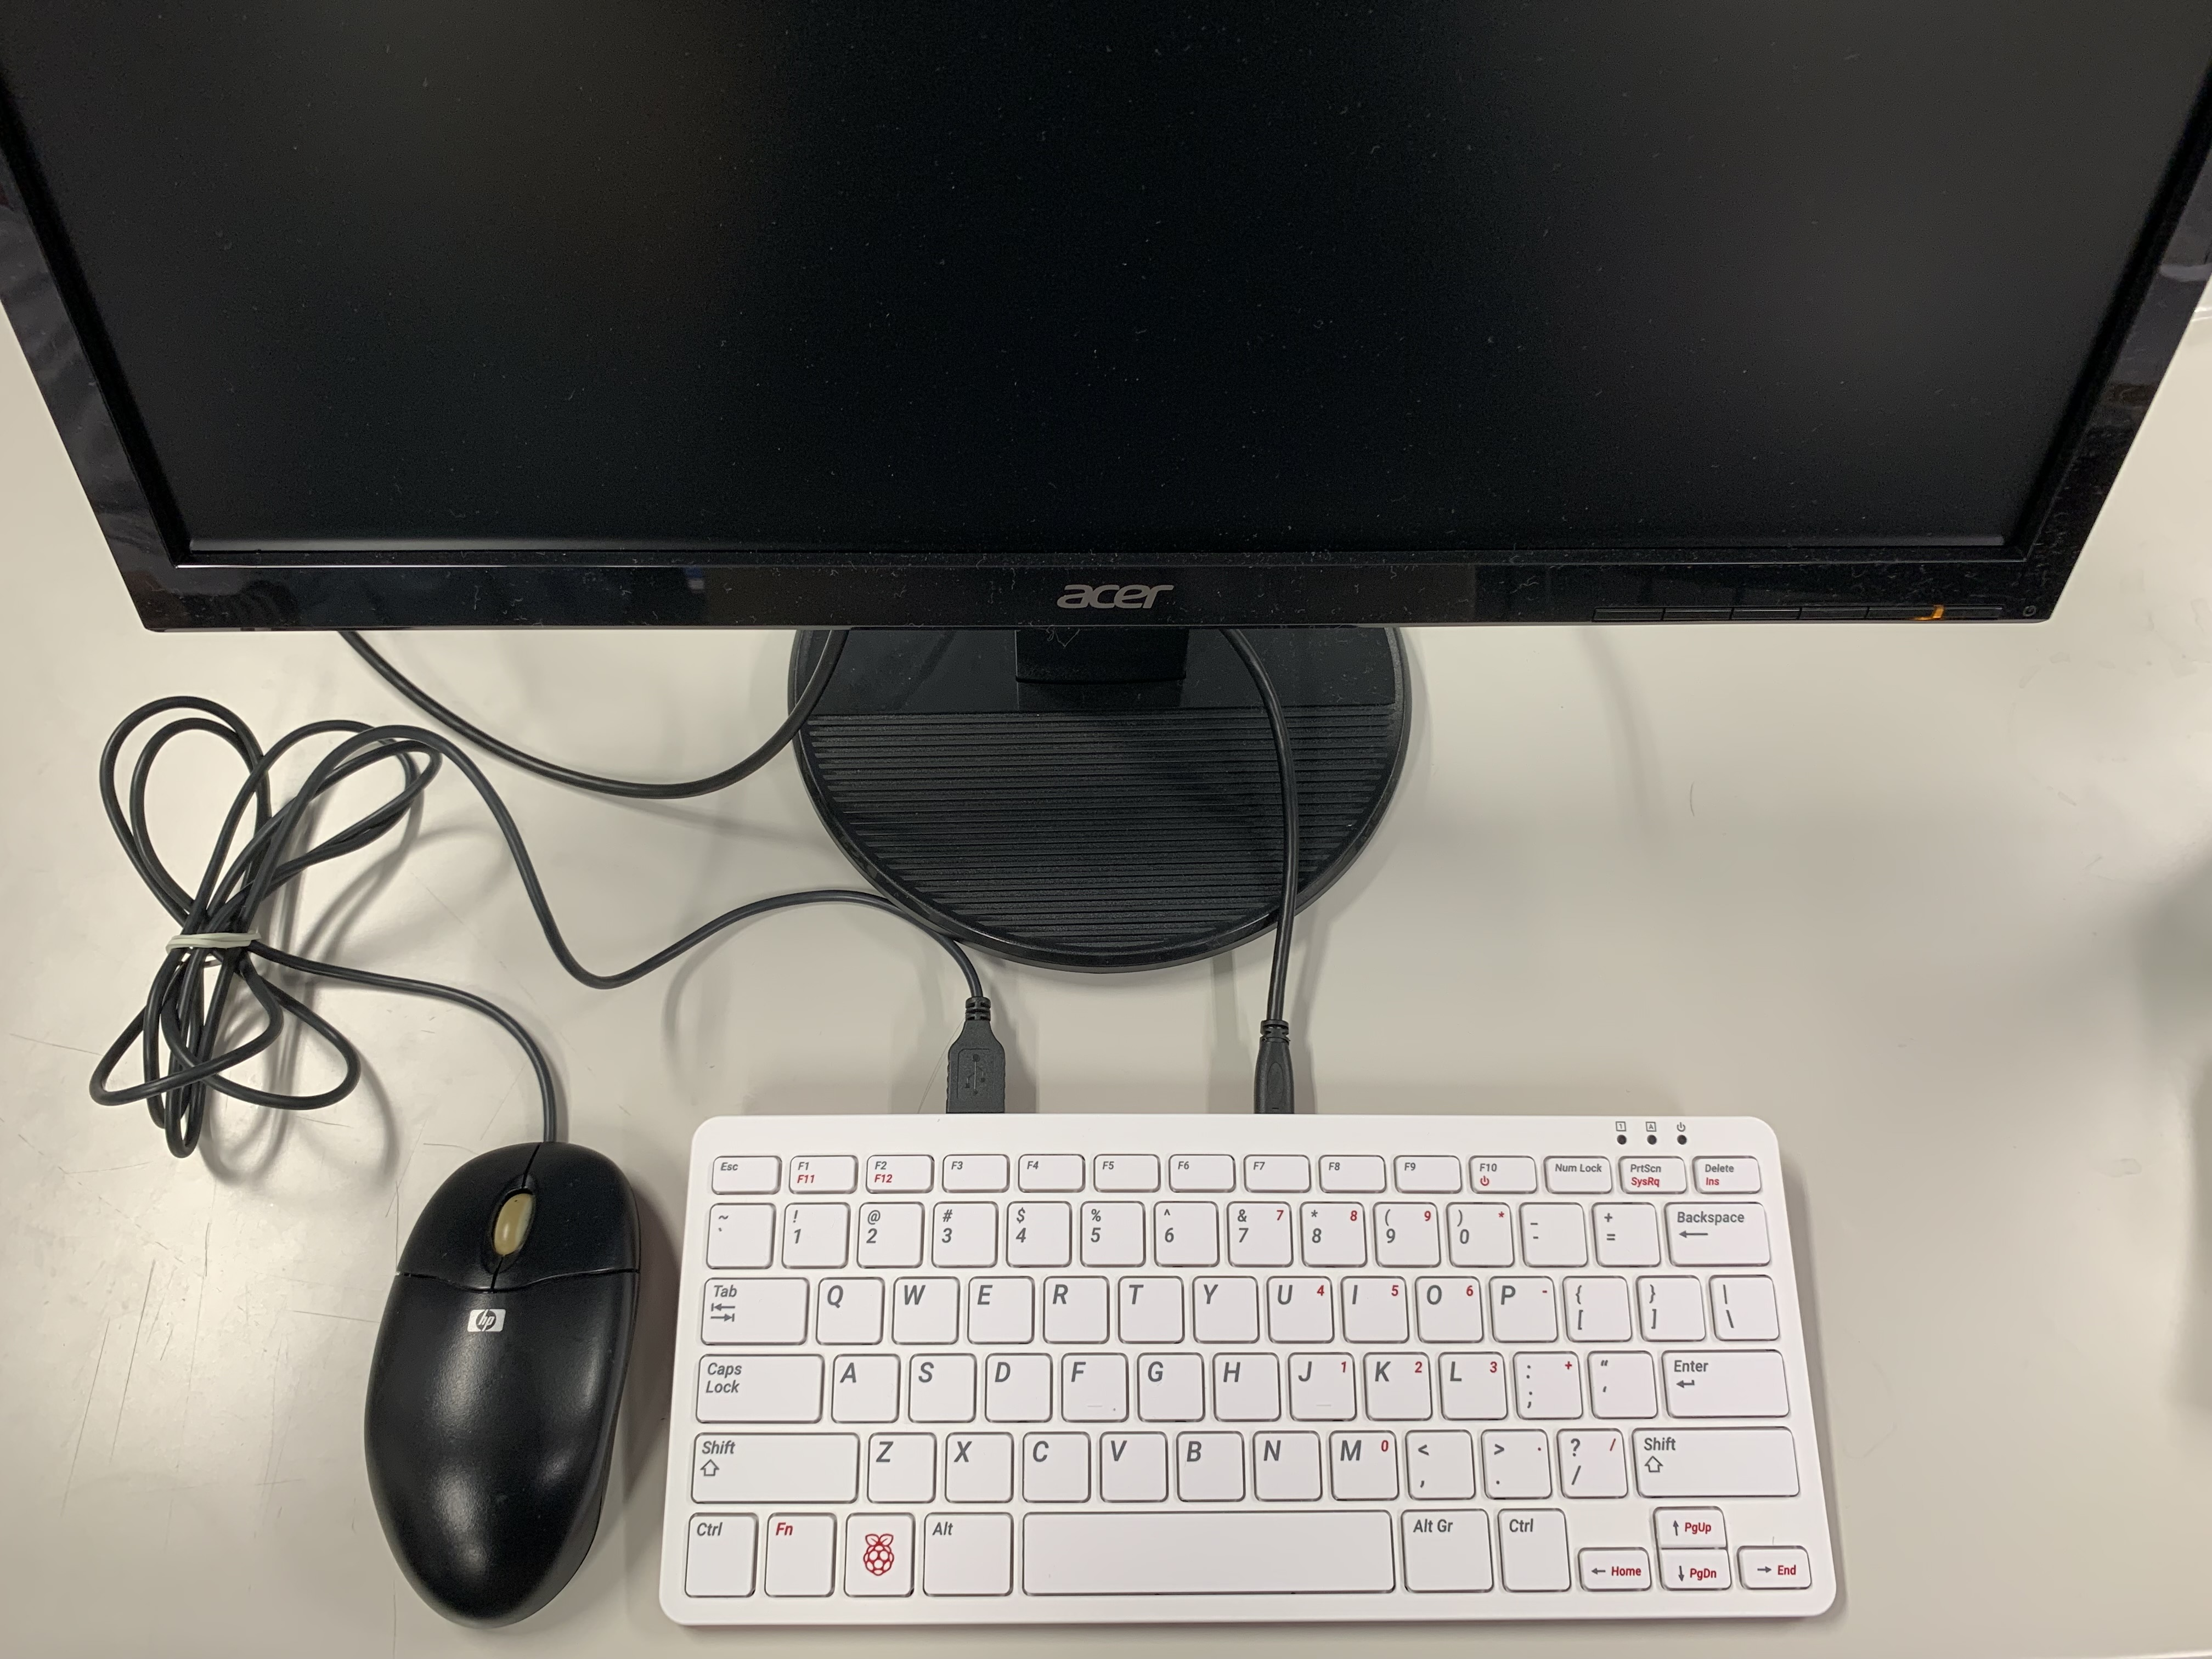
\includegraphics[width=0.8\linewidth]{connections01-2023.jpg}
      \newline
      \stepcounter{Figure}{\theFigure}: \ruby{接続}{せつぞく}の全体図}

  \end{minipage}
\end{figure}

%\liststyleLxii
\begin{enumerate}
  \item ラズベリーパイとモニタをつなぐ

        \begin{itemize}
          \item
                ラズベリーパイとモニタをHDMIケーブルで\ruby{接続}{せつぞく}します。右側のHDMIポートを使用してください。~\ref{seq:refFigure1}、~\ref{seq:refFigure2}を参考にしてください。お家でやる場合は、モニタもしくはTVによってはHDMIの\ruby{差し込み}{さしこみ}口の場所が\ruby{異}{こと}なる場合があります。説明書等を\ruby{別途}{べっと}参照してください\textbf{。}


                \begin{figure}[h]
		\centering
                  \begin{minipage}{0.45\textwidth}
                    {\upshape
                      %[Warning: Image ignored] % Unhandled or unsupported graphics:
                      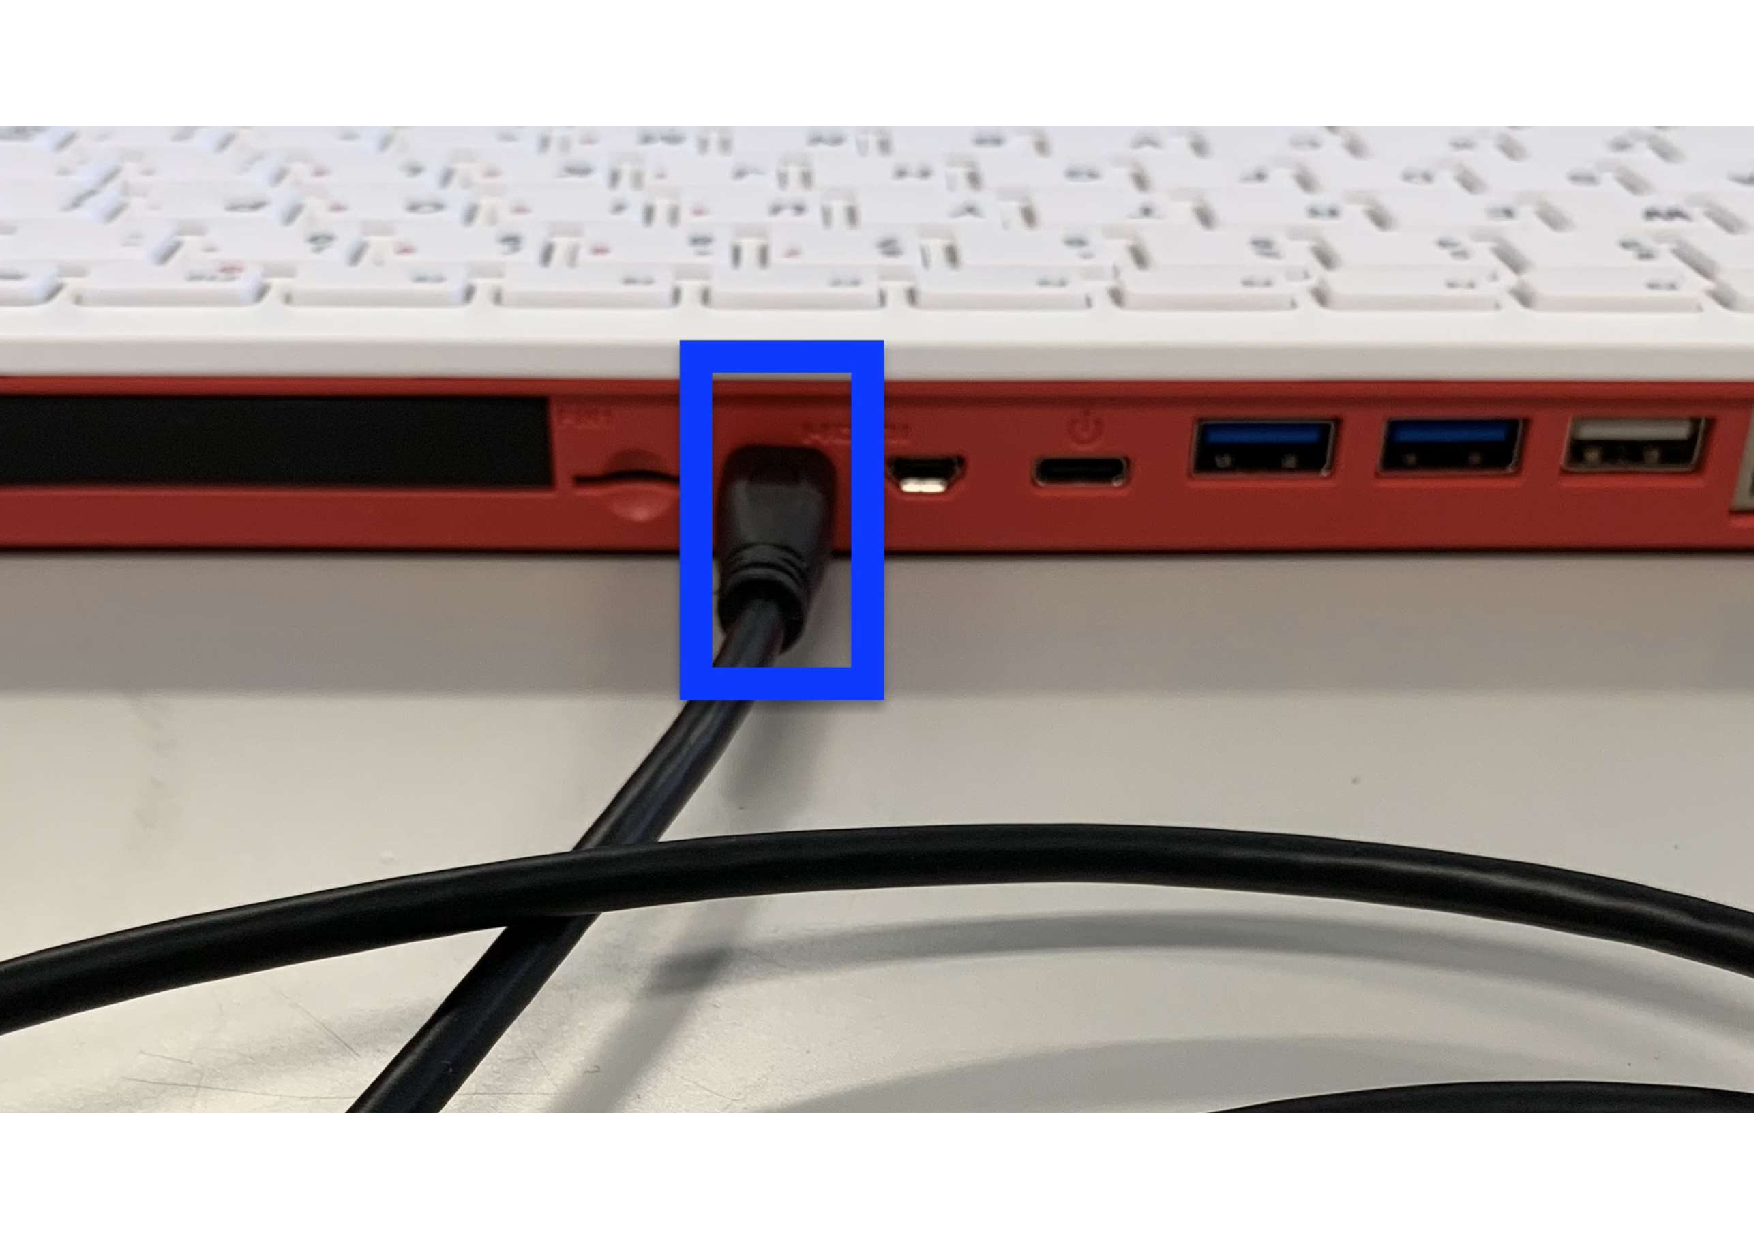
\includegraphics[height=3.471cm]{figure222023.pdf}
                      \newline
                      {\refstepcounter{Figure}\theFigure\label{seq:refFigure1}}:
                      ラズベリーパイHDMI\ruby{接続}{せつぞく}}
                  \end{minipage}
		\centering
                  \begin{minipage}{0.45\textwidth}
                    {\upshape
                      %[Warning: Image ignored] % Unhandled or unsupported graphics:
                      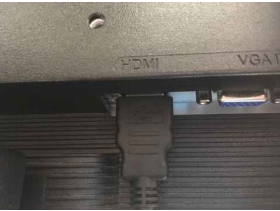
\includegraphics[height=3.471cm]{textbook-img016.png}
                      \newline
                      {\refstepcounter{Figure}\theFigure\label{seq:refFigure2}}:
                      ディスプレイHDMI\ruby{接続}{せつぞく}}
                  \end{minipage}
                \end{figure}

        \end{itemize}
  \item マウスをつなぐ

        \begin{itemize}
          \item
                マウスの先をラズベリーパイへ差し\ruby{込}{こ}みます。
        \end{itemize}
\end{enumerate}

\begin{figure}[h]
  \centering
  \begin{minipage}{0.5\textwidth}
    {\upshape
      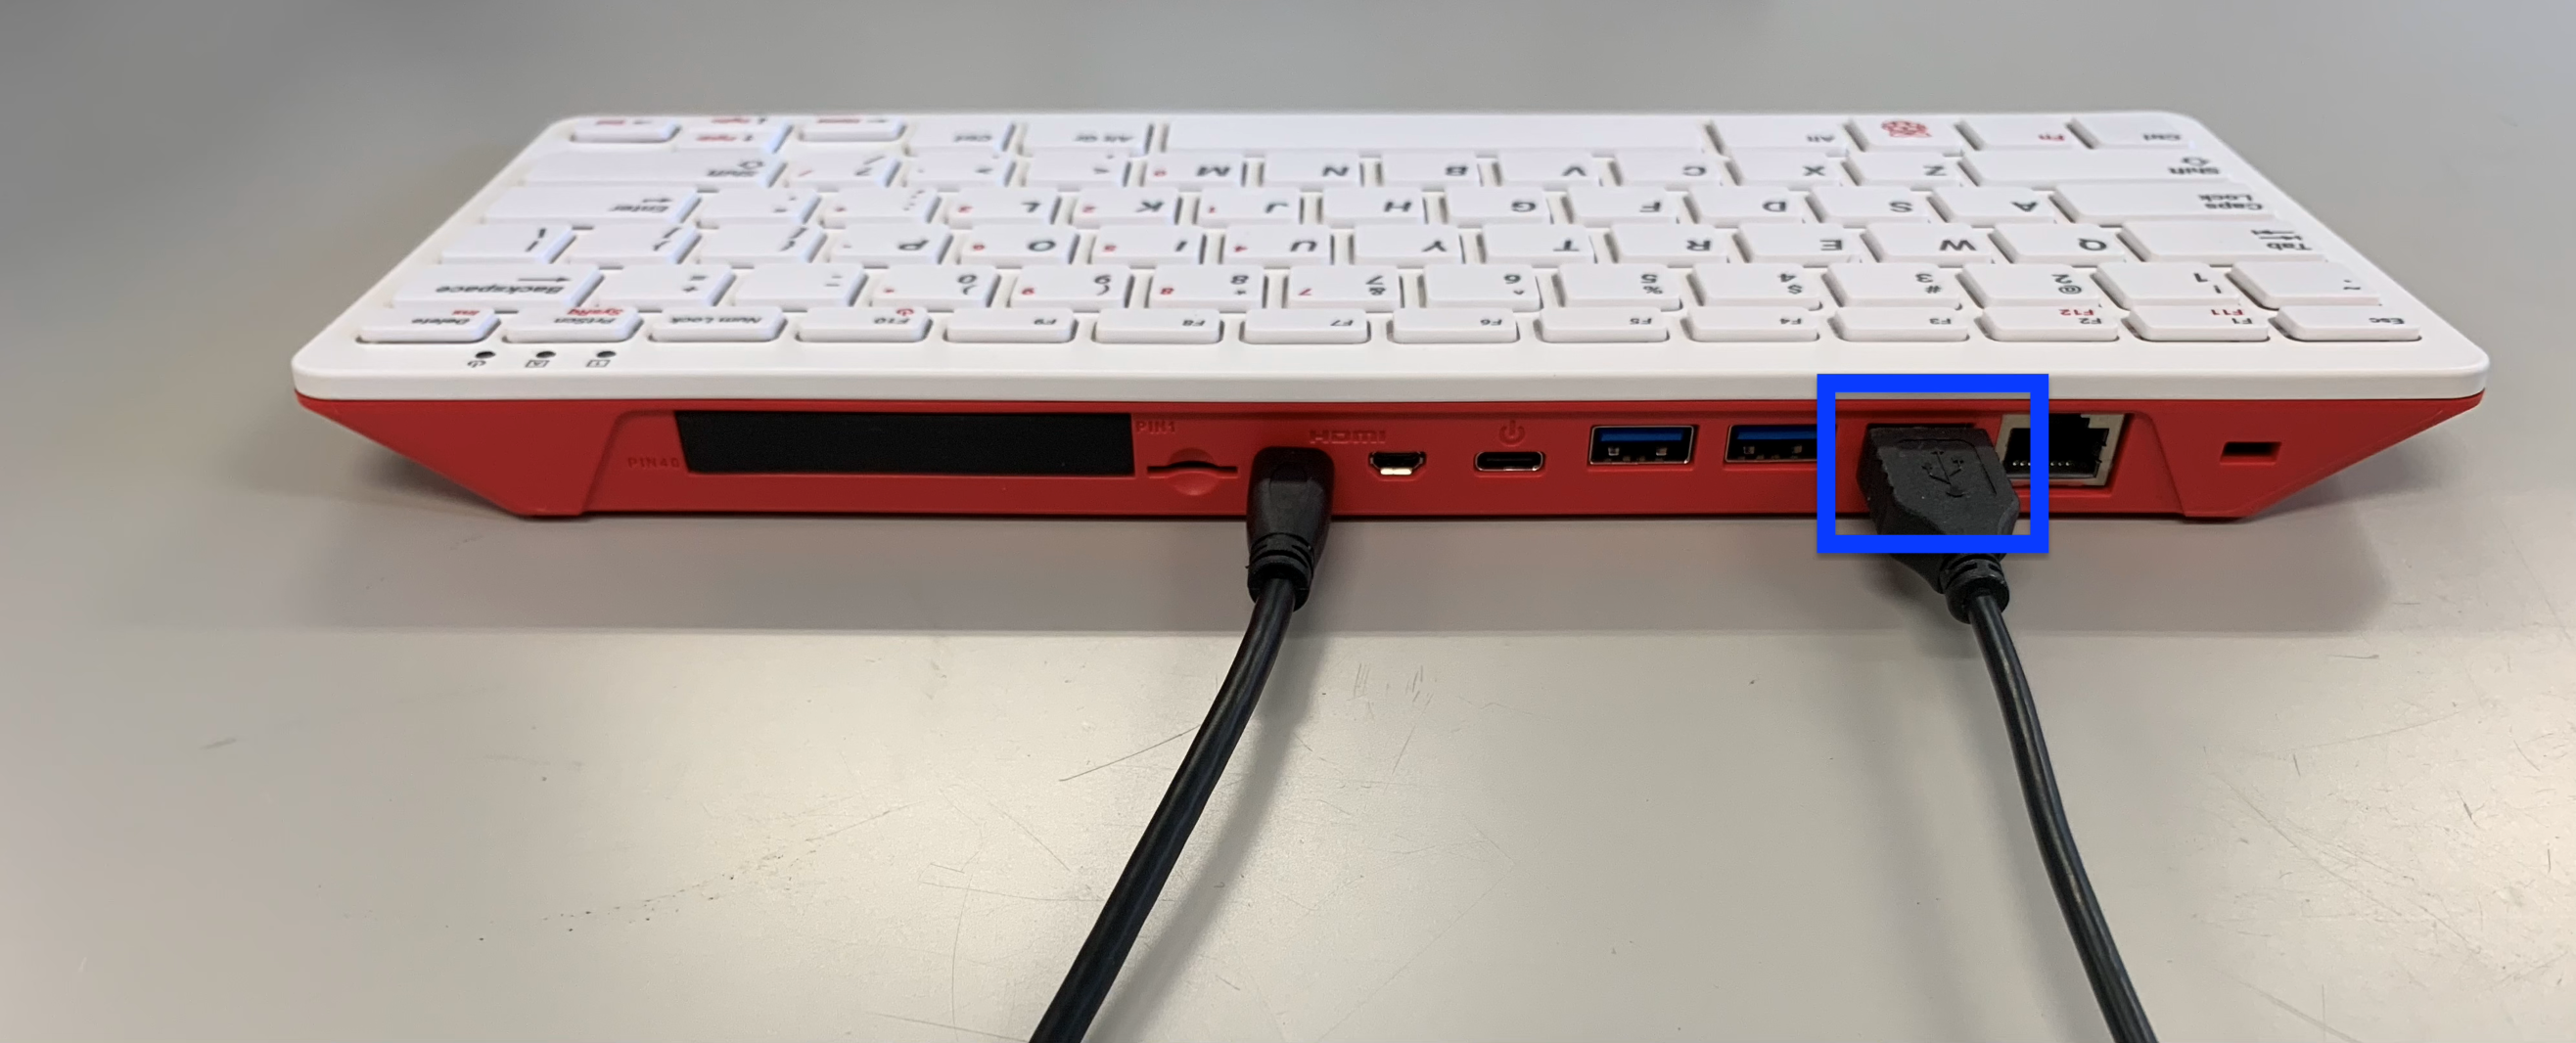
\includegraphics[width=\linewidth]{figure1.10-4.png}
      \newline
      Figure \stepcounter{Figure}{\theFigure}:
      マウスの\ruby{接続}{せつぞく}}
  \end{minipage}
\end{figure}
%\liststyleLxii
\setcounter{saveenum}{\value{enumi}}
\begin{enumerate}
  \setcounter{enumi}{\value{saveenum}}
  \clearpage
  \item
        microSD(マイクロエスディー)
        カードをいれる

        \begin{itemize}
          \item
                microSDカードをラズベリーパイ本体にさします。小さいのでなくさないように気をつけましょう。

                \begin{figure}[h]
                  \centering
                  \begin{minipage}{0.45\textwidth}
                    {\upshape
                      \includegraphics[width=0.8\linewidth]{figure1.10-5.png}
                      \newline
                      \stepcounter{Figure}{\theFigure}: microSDカードのさしこみ}
                  \end{minipage}
                \end{figure}

                \bigskip
        \end{itemize}
  \item モニタのでんげんをいれる

        \begin{itemize}
          \item
                次にモニタのコンセントをさします。モニタのみぎはじのボタンをおします。でんげんが入ると青色にてんとうします。お家でやるときはでんげんのいれた後、入力きりかえが必要となる場合がありますので、説明書等を\ruby{別途}{べっと}参照してください。


                \begin{figure}[h]
                  \centering
                  \begin{minipage}{0.45\textwidth}
                    {\upshape
                      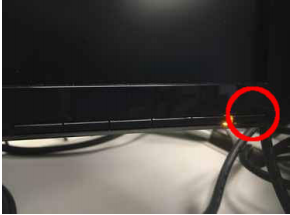
\includegraphics[width=0.8\linewidth]{textbook-img019.png}
                      \newline
                      \stepcounter{Figure}{\theFigure}:
                      モニタでんげんボタンの位置}
                  \end{minipage}
                \end{figure}
        \end{itemize}
  \item ラズベリーパイのでんげんをいれる

        \begin{itemize}
          \item
                最後にラズベリーパイのでんげんをいれます。~\ref{seq:refFigure6}のようにラズベリーパイにでんげんケーブルをさしてコンセントへ\ruby{接続}{せつぞく}します。緑色のランプがついてディスプレイにラズベリーが\ruby{表示}{ひょうじ}がされます~\ref{seq:refFigure7}。
        \end{itemize}

        \centering
        \begin{minipage}{\textwidth}
          \begin{minipage}{0.45\textwidth}
            \centering
            {\upshape
              \centering
              \includegraphics[width=0.8\linewidth]{textbook-img020-2023.png}
              \newline
              {\refstepcounter{Figure}\theFigure\label{seq:refFigure6}}:
              ラズベリーパイでんげん\ruby{接続}{せつぞく}}
          \end{minipage}
          \begin{minipage}{0.45\textwidth}
            \centering
            {\upshape
              \centering
              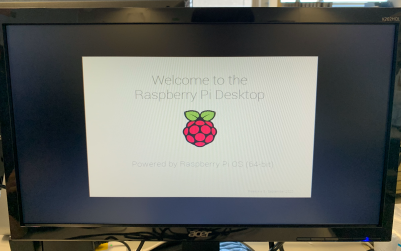
\includegraphics[width=0.8\linewidth]{textbook-img0212023.png}
              \newline
              {\refstepcounter{Figure}\theFigure\label{seq:refFigure7}}:
              ラズベリーパイ起動中}
            \end{minipage}
          \end{minipage}


\clearpage
\end{enumerate}


\refstepcounter{Exercise}
  \subsection{\theExercise  セットアップをしよう}
  \item  定住国を\ruby{設定}{せってい}して言語とタイムゾーンを決定しよう
        \begin{itemize}
          \item
                raspberry pi 400 が起動すると,このような~\ref{seq:refFigure8}セットアップの開始画面になります。この画面ではそのままNextのボタンを\ruby{押}{お}して次に進みます。
        \end{itemize}
        \begin{figure}[h]
          \centering
          \begin{minipage}{0.5\textwidth}
          {\upshape
            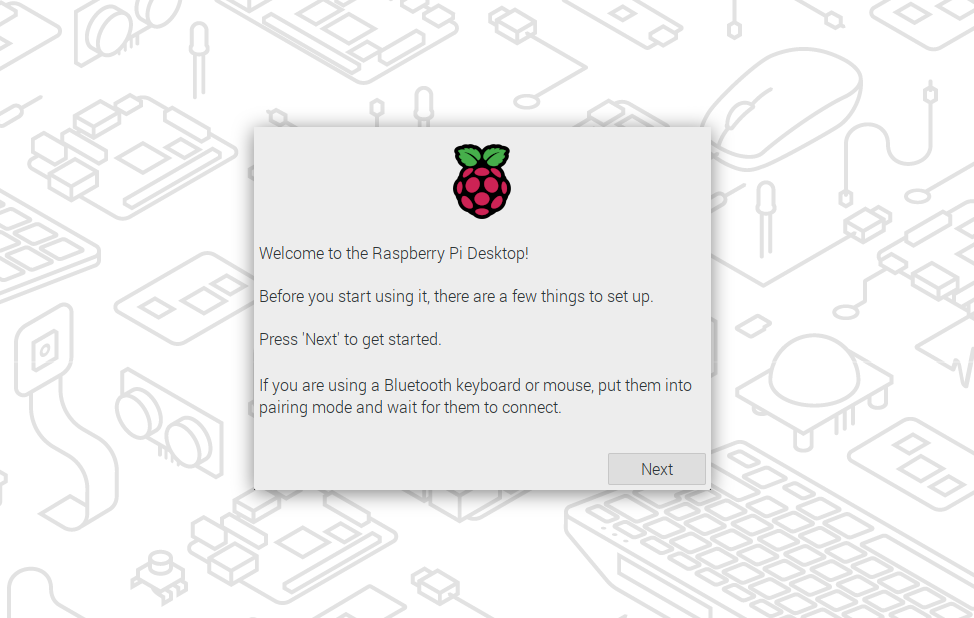
\includegraphics[width=0.9\linewidth]{sw_image01.png}
            \newline
            {\refstepcounter{Figure}\theFigure\label{seq:refFigure8}}:
            起動後画面
          }
        \end{minipage}
        \end{figure}

        \begin{itemize}
          \item
              次の画面では~\ref{seq:refFigure9}のように自分の住んでいる\ruby{地域}{ちいき}(タイムゾーン)を\ruby{設定}{せってい}することで言語や時間を決定することができます。今回は\ruby{皆}{みな}さん日本に住んでいると思うのでcountryの行をクリックすると~\ref{seq:refFigure10}のように\ruby{様々}{さまざま}な国の名前が\ruby{表示}{ひょうじ}されるのでその中からJapanを\ruby{選択}{せんたく}してください。そうすると他のLanguage, Timezoneの\ruby{項目}{こうもく}がjapanese,Tokyoになります。これらはそれぞれ言語とタイムゾーンを表しています。それぞれJapan,japanese, Tokyoになっていることとピンクの\ruby{枠}{わく}の場所にチェックが入っていることを\ruby{確認}{かくにん}できたらNextボタンを\ruby{押}{お}します。
              
              
                \begin{figure}[h]
                \centering
                \begin{minipage}{0.45\textwidth}
                  {\upshape
                    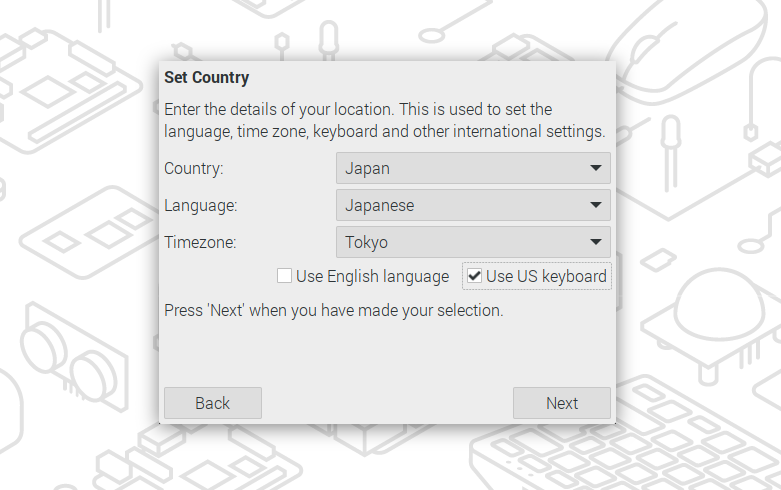
\includegraphics[width=\linewidth]{sw_image02.png}
                    \newline
                    {\refstepcounter{Figure}\theFigure\label{seq:refFigure9}}:
                    タイムゾーン画面}
                \end{minipage}
                \hfill
                \centering
                \begin{minipage}{0.45\textwidth}
                  {\upshape
                    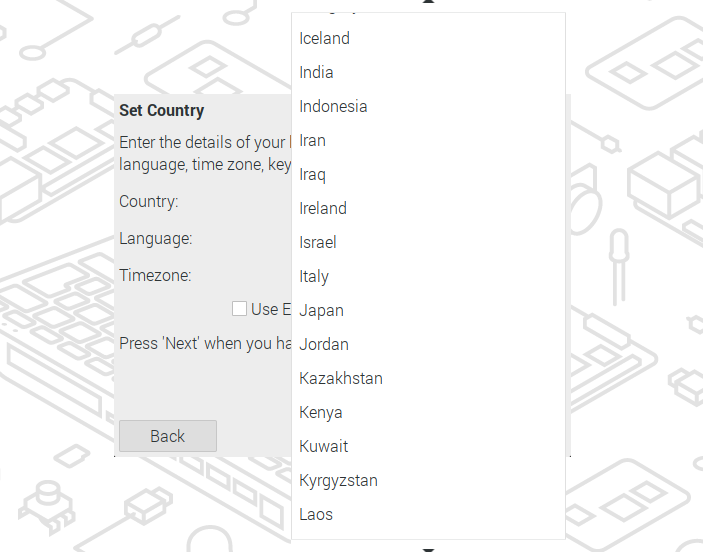
\includegraphics[width=\linewidth]{sw_image03-2.png}
                    \newline
                    {\refstepcounter{Figure}\theFigure\label{seq:refFigure10}}:
                    \ruby{選択}{せんたく}画面}
                \end{minipage}
              \end{figure}   
              \item   注意点として\ruby{未来塾}{みらいじゅく}で使用するキーボードの配列について\ruby{日常的}{にちじょうてき}に日本で使用されているキーボードの配列とは\ruby{異}{こと}なるコンピュータの\ruby{専門家}{せんもんか}に多く使われている米国のUS配列というキーボードを用いています。キーボードの\ruby{並}{なら}びは国や\ruby{規格}{きかく}、機械などによってそれぞれ\ruby{異}{こと}なった形を持つものがあるので注意してください。 
        \end{itemize}   
        \clearpage 

  \refstepcounter{Exercise}    
  \subsection{\theExercise パスワードとユーザー名(ID)を決めよう}         
          
                \begin{itemize}
                \item                                      
                次にユーザーを作成します。~\ref{seq:refFigure11}のように上から順にユーザー名、パスワード、\ruby{再度}{さいど}入力用パスワードの入力の順になっています。
              
        
                    \begin{figure}[h]
                      \centering
                      \begin{minipage}{5.228cm}
                        {\upshape
                          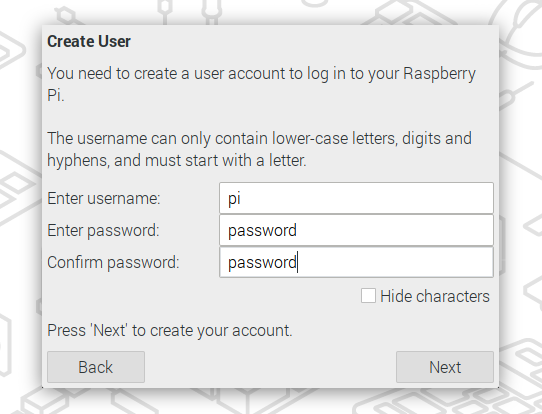
\includegraphics[width=6.000cm]{sw_image03.png}
                          \newline
                          {\refstepcounter{Figure}\theFigure\label{seq:refFigure11}}:
                          ユーザー作成}
                      \end{minipage}
                    \end{figure}
                  \end{itemize}
                  \begin{itemize}
                  \item
                      先ほど記入したものを\ruby{実際}{じっさい}に入力してみます。その\ruby{際}{さい}にこのような画面Figure~\ref{seq:refFigure14}が出てきたらユーザー名(ID)かパスワードのどれかに不正な文字などが\ruby{含}{ふく}まれている\ruby{可能性}{かのうせい}があるのでもう一度\ruby{確認}{かくにん}しましょう。
                      \begin{figure}[h]
                        \centering
                        \begin{minipage}{5.228cm}
                          {\upshape
                            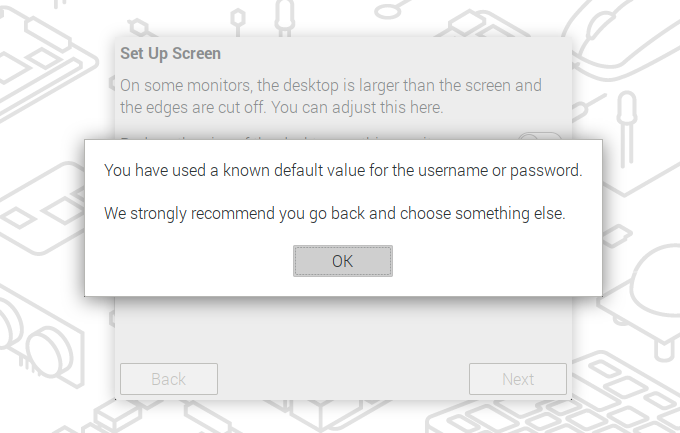
\includegraphics[width=6.000cm]{sw_image04.png}
                            \newline
                            {\refstepcounter{Figure}\theFigure\label{seq:refFigure14}}:
                            エラー画面}
                        \end{minipage}
                      \end{figure}
                \end{itemize}
                \begin{itemize}
                  \item
                        次にスクリーンサイズをTAの人と画面が\ruby{歪}{ゆが}んだりしていないか、\ruby{縦横}{たてよこ}に\ruby{伸}{の}びていないかを\ruby{一緒}{いっしょ}に\ruby{確認}{かくにん}してください。問題の無い場合はNextを\ruby{押}{お}して次に進みます。~\ref{seq:refFigure15}
                        \begin{figure}[h]
                          \centering
                          \begin{minipage}{5.228cm}
                            {\upshape
                              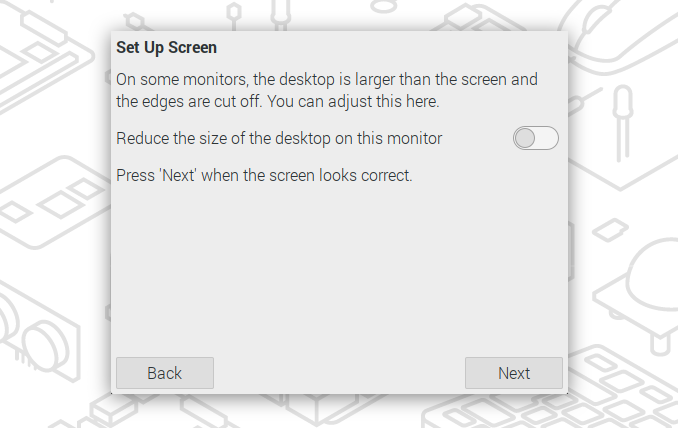
\includegraphics[width=6.000cm]{sw_image05.png}
                              \newline
                              {\refstepcounter{Figure}\theFigure\label{seq:refFigure15}}:
                              スクリーンサイズ\ruby{確認}{かくにん}}
                          \end{minipage}
                        \end{figure}
                      \end{itemize}  
                      
  \clearpage                   
  \refstepcounter{Exercise}
    \subsection{\theExercise Wi-Fiを\ruby{接続}{せつぞく}しよう}
                \begin{itemize}
                  \item
                        次にWi-Fiの\ruby{設定}{せってい}を行います。この\ruby{赤枠}{あかわく}の中に\ruby{接続可能}{せつぞくかのう}なWi-Fiの名前が\ruby{表示}{ひょうじ}されます。~\ref{seq:refFigure16}
                        \item
                        \refstepcounter{Question}\theQuestion またこのセクションではWi-FIのアドレスとパスワードが必要となるのでTA(ティーチングアシスタント(Teaching Assistant))の人からアドレスとパスワードを教えてもらい、下の\ruby{欄}{らん}に記入しておきましょう。
                        \addBlank{Wi-Fiアドレス}
                        \addBlank{パスワード}
                        \item
                        上部で記入したアドレスを\ruby{選択}{せんたく}してNextのボタンを\ruby{押}{お}します。
                        \begin{figure}[h]
                          \centering
                          \begin{minipage}{5.228cm}
                            {\upshape
                              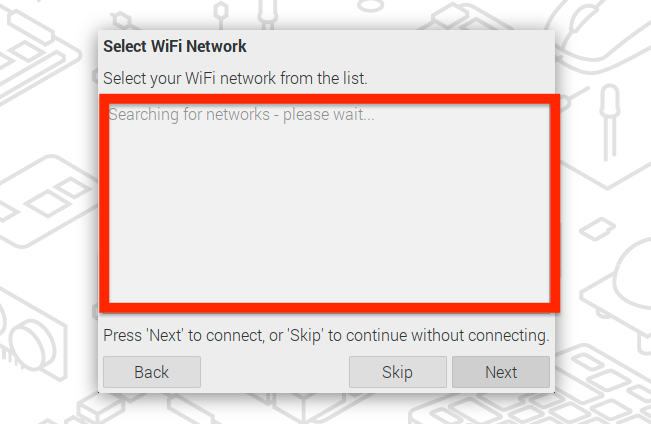
\includegraphics[width=7.000cm]{sw_image06kai.png}
                              \newline
                              {\refstepcounter{Figure}\theFigure\label{seq:refFigure16}}:
                              Wi-Fi\ruby{設定}{せってい}}
                          \end{minipage}
                        \end{figure}
                \end{itemize}
                \begin{itemize}
                  \item
                      そうするとパスワードを入力するように求められます。 ここでも上部で記入したパスワードを入力してNextを\ruby{押}{お}します。
                      \begin{figure}[h]
                        \centering
                        \begin{minipage}{5.228cm}
                          {\upshape
                            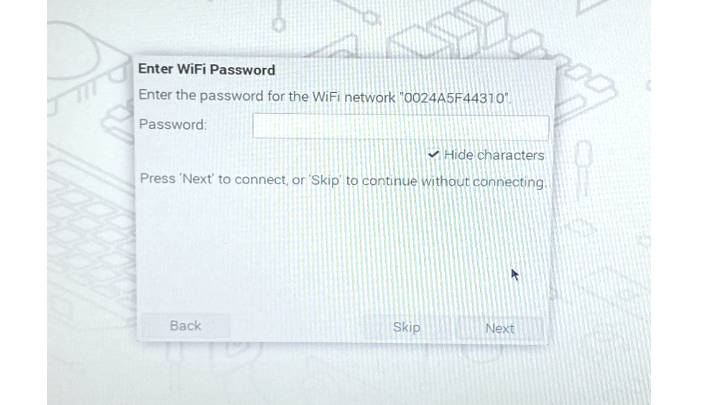
\includegraphics[width=9.000cm]{pswd_image_0404.png}
                            \newline
                            {\refstepcounter{Figure}\theFigure\label{seq:refFigure17}}:
                            パスワード入力}
                        \end{minipage}
                      \end{figure}
                      
                \end{itemize}  
   \clearpage
   \refstepcounter{Exercise}     
   \subsection{\theExercise  アップデートをスキップしてraspberry piを始めよう}   
    \item
        アップデートをスキップしよう
                \begin{itemize}
                  \item
                      次の画面に進むとソフトウェアアップデートを求められますが、\textbf{今回はアップデートをしないでください。~\ref{seq:refFigure18}の}\textbf{\color{red}赤い枠のSkipボタン}を\ruby{押}{お}して次の画面に\ruby{移動}{いどう}します。
                      \begin{figure}[h]
                        \centering
                        \begin{minipage}{5.228cm}
                          {\upshape
                            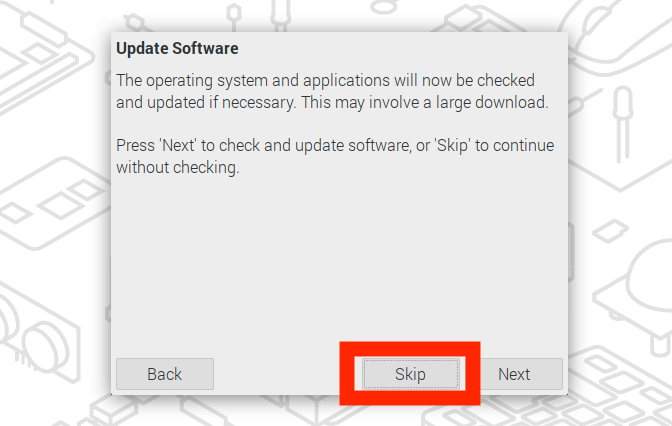
\includegraphics[width=7.000cm]{sw_image07.png}
                            \newline
                            {\refstepcounter{Figure}\theFigure\label{seq:refFigure18}}:
                            ソフトウェアアップデート}
                        \end{minipage}
                      \end{figure}
                      \\ここでアップデートをしてしまうと、\ruby{授業}{じゅぎょう}で使う教材の一部が正しく動かなくなってしまいます。
                      もし、\ruby{間違}{まちが}えてアップデートをしてしまった場合には、
                      SDカードの\ruby{交換}{こうかん}をする必要があるので、すぐにグループの先生に\ruby{相談}{そうだん}してください。
                      \bigskip
                  \end{itemize}  
    \item
        \ruby{再起動}{さいきどう}をしてraspberry piを始めよう
                \begin{itemize}
                  \item
                        次に大まかな初期\ruby{設定}{せってい}が\ruby{完了}{かんりょう}したので\ruby{再起動}{さいきどう}を行います。画面右下にあるRestartのボタンを\ruby{押}{お}してください。そうすると\ruby{再起動}{さいきどう}が開始されます。
                        \begin{figure}[h]
                          \centering
                          \begin{minipage}{5.228cm}
                            {\upshape
                              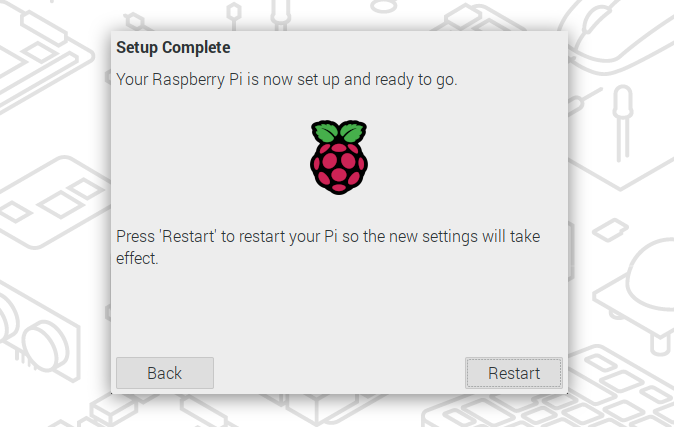
\includegraphics[width=7.000cm]{sw_image08.png}
                              \newline
                              {\refstepcounter{Figure}\theFigure\label{seq:refFigure19}}:
                              \ruby{再起動}{さいきどう} }
                          \end{minipage}
                        \end{figure}
                  \end{itemize}

\clearpage
\end{enumerate}
\end{document}
